\documentclass[12pt]{article}
\usepackage[swedish,english]{babel}
\usepackage[utf8x]{inputenc}
\usepackage{amsmath}
\usepackage{graphicx}
\usepackage{float} %for insert graph
\usepackage{lscape}
\usepackage{rotating}
\usepackage[colorinlistoftodos]{todonotes}
%\usepackage[margin=1in]{geometry} %set page margin
\usepackage[bottom=1.25in, top=1.25in]{geometry}
%\addtolength{\topmargin}{0.25in}
%\addtolength{\bottommargin}{0.25in}
\usepackage{hyperref} %insert to link to email address
\usepackage{setspace}
\setlength\parindent{24pt} %set indentation
\usepackage{amssymb} %for maths symbols
\usepackage{cases} %for numbering in cases
  %define matlab style
\usepackage{listings}
\usepackage{color} %red, green, blue, yellow, cyan, magenta, black, white
\definecolor{mygreen}{RGB}{28,172,0} % color values Red, Green, Blue
\definecolor{mylilas}{RGB}{170,55,241}
\usepackage{grffile} %to avoid showing the file names of figures

\lstset{language=Matlab,%
    %basicstyle=\color{red},
    breaklines=true,%
    morekeywords={matlab2tikz},
    keywordstyle=\color{blue},%
    morekeywords=[2]{1}, keywordstyle=[2]{\color{black}},
    identifierstyle=\color{black},%
    stringstyle=\color{mylilas},
    commentstyle=\color{mygreen},%
    showstringspaces=false,%without this there will be a symbol in the places where there is a space
    numbers=left,%
    numberstyle={\tiny \color{black}}% size of the numbers
    %numbersep=9pt, % this defines how far the numbers are from the text
    %emph=[1]{for,end,break},emphstyle=[1]\color{red}, %some words to emphasise
    %emph=[2]{word1,word2}, emphstyle=[2]{style},    
}


\begin{document}

%%%%%%%%%%%
%%TITLE PAGE%%%
%%%%%%%%%%%%
\begin{titlepage}

\newcommand{\HRule}{\rule{\linewidth}{0.5mm}} % Defines a new command for the horizontal lines, change thickness here

\center % Center everything on the page
 
%----------------------------------------------------------------------------------------
%   HEADING SECTIONS
%----------------------------------------------------------------------------------------
%Logo First
%----------------------------------------------------------------------------------------
%   LOGO SECTION
%----------------------------------------------------------------------------------------


\includegraphics{UU_logo.eps}\\[0.5cm] % Include a department/university logo - this will require the graphicx package
 
\textsc{\huge Modelling complex systems}\\[0.5cm] % Major heading such as course name


%----------------------------------------------------------------------------------------
%   TITLE SECTION
%----------------------------------------------------------------------------------------

\HRule \\[0.4cm]
{\huge \bfseries Project 2}\\[0.2cm] % Title of your document
{\Large Population Dynamics \par Groups of Friends \par Network Epidemics \par Flocks and Predators }
\\

\HRule \\[0.4cm]
%{\Large Population Dynamics \par Groups of Friends \par Network Epidemics \par Flocks and Predators }

 
%----------------------------------------------------------------------------------------
%   AUTHOR SECTION
%----------------------------------------------------------------------------------------

{\huge Peili Guo\\} %insert your name 
{\large \href{mailto:Peili.Guo.7645@student.uu.se}{Peili.Guo.7645@student.uu.se}}
\\[2cm] %insert page break length

%----------------------------------------------------------------------------------------
%   DATE SECTION
%----------------------------------------------------------------------------------------

{\Large \today}\\[2cm] % Date, change the \today to a set date if you want to be precise


%----------------------------------------------------------------------------------------

\vfill % Fill the rest of the page with whitespace

\end{titlepage}

\newpage
%%%%%%%%%%%%
%%%start report 
%%%1. population dynamics
%%%%%%%%%%%

\section{Population Dynamics}
\doublespacing
In this part, we model the population with a stochastic model. There are n resource sites in the model world, and at time t =0, the population is $A_{0}$ and they are assigned randomly to one resource site. At each t step, the population rules are, if there are exactly two individuals on the same site. They reproduce b offsprings and these offsprings are assigned randomly to resources sites. If the number of individuals on a resources sites is any number other than 2, no offspring will be reproduced. 

\subsection{Matlab model}

To begin, we can run this with different parameters and simulate in Matlab and observe the total number of population at different time step. The different parameters are: 

\begin{enumerate}
\item b: number of offspring if reproduce
\item n: total of number of resource sites
\item $A_{0}$: initial population
\item t: the time steps we want to simulate the model
\end{enumerate}


When set the initial population to a small number relative to the resource site, it would be difficult to have 2 individuals at the same site for reproduce, and even if they reproduce a large number of offspring the population dies out very quick. 
below are some plots showing the total number of population at different time steps with different parameters. 

\begin{figure}[H] %figure 1 at x0=10 b= 50
\centering
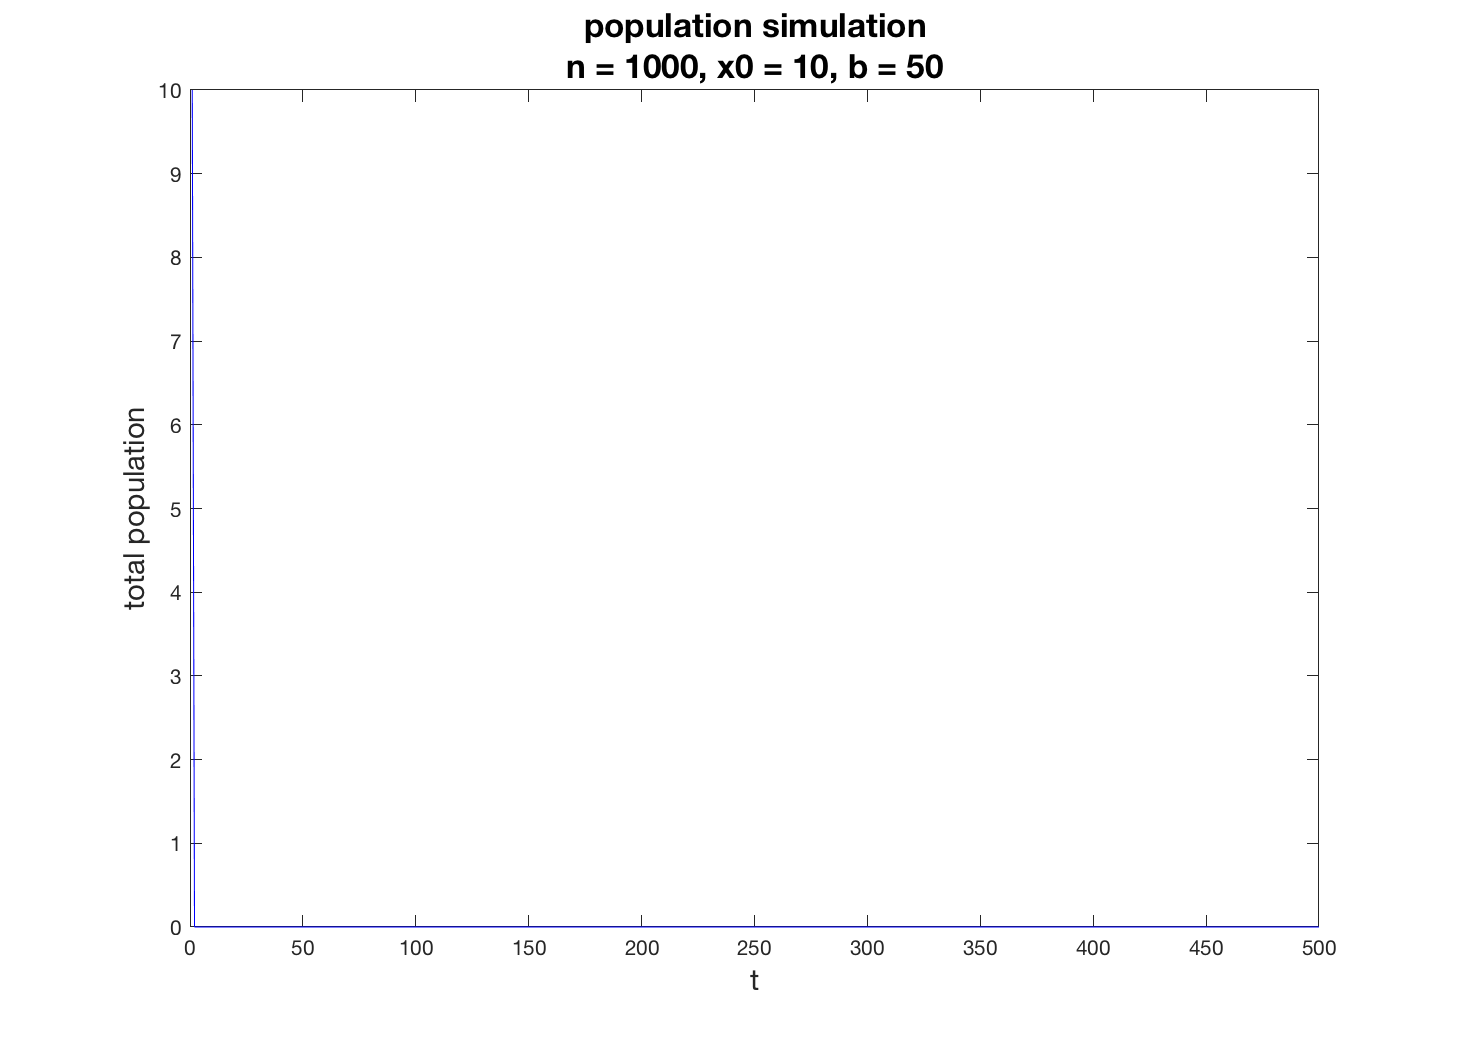
\includegraphics[width = 12 cm, height = 9cm]{single_run n1000 x010 b50.png}
\caption{initial population of 10 b = 50 not reproducing}
\label{fig:p1s1}
\end{figure}

\begin{figure}[H] %figure 2 x0 = 50 b =30 
\centering
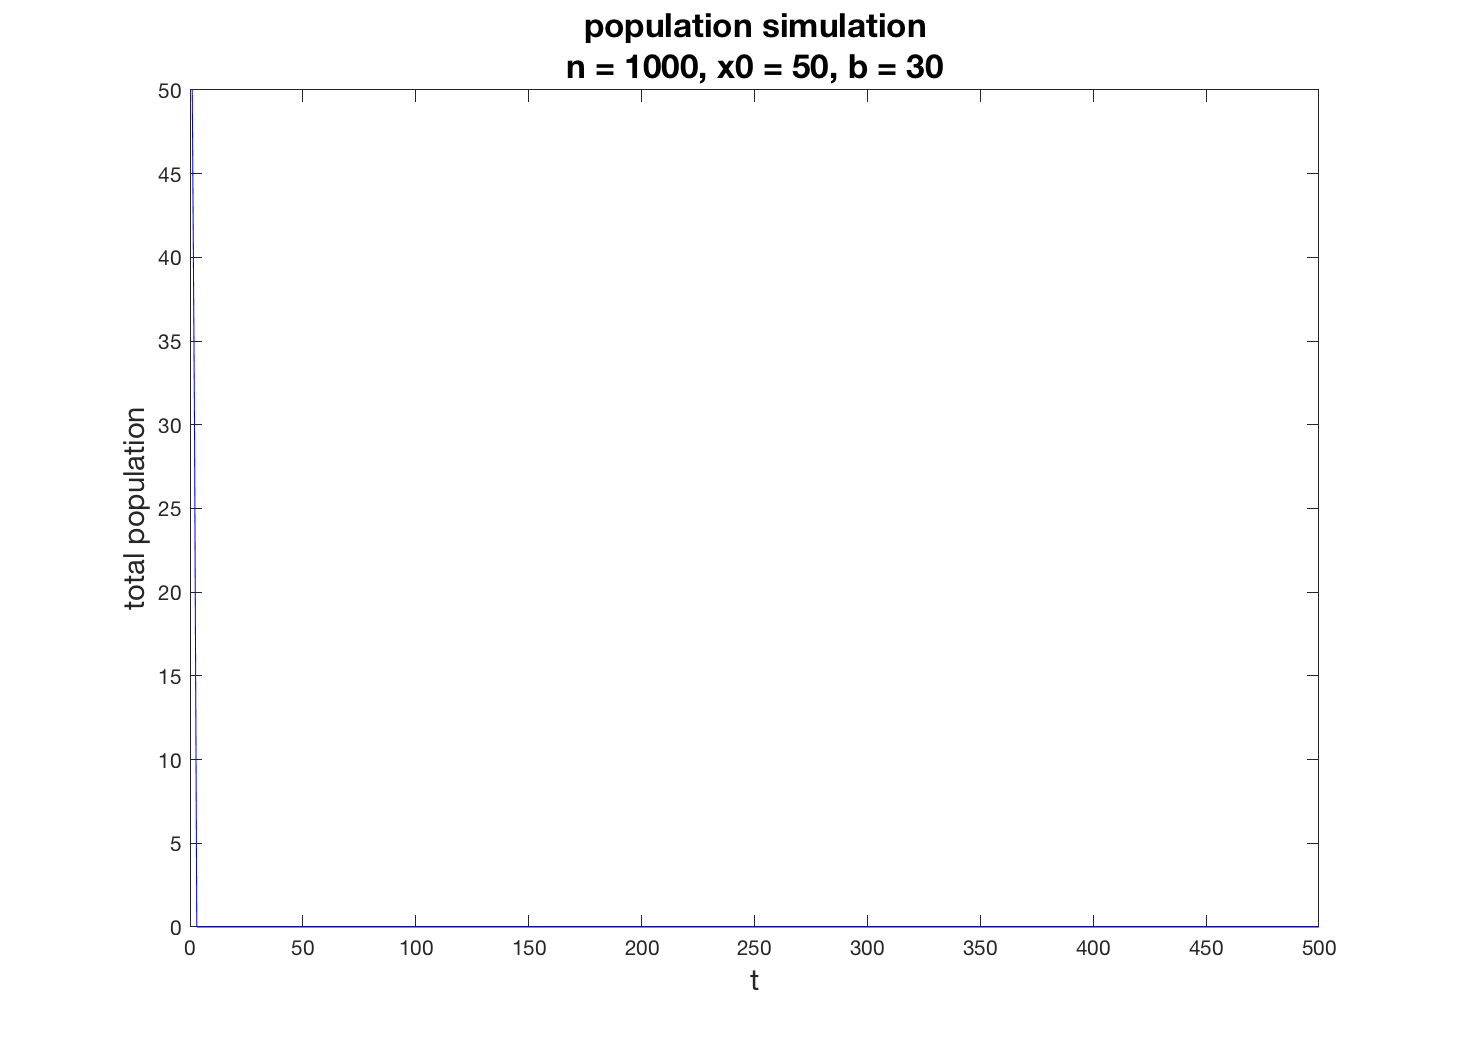
\includegraphics[width = 12 cm, height = 9cm]{single_run n1000 x050 b30.png}
\caption{initial population of 50 and b =30 not reproducing}
\label{fig:p1s2}
\end{figure}

\begin{figure}[H] %figure3 x0 = 50 b= 50
\centering
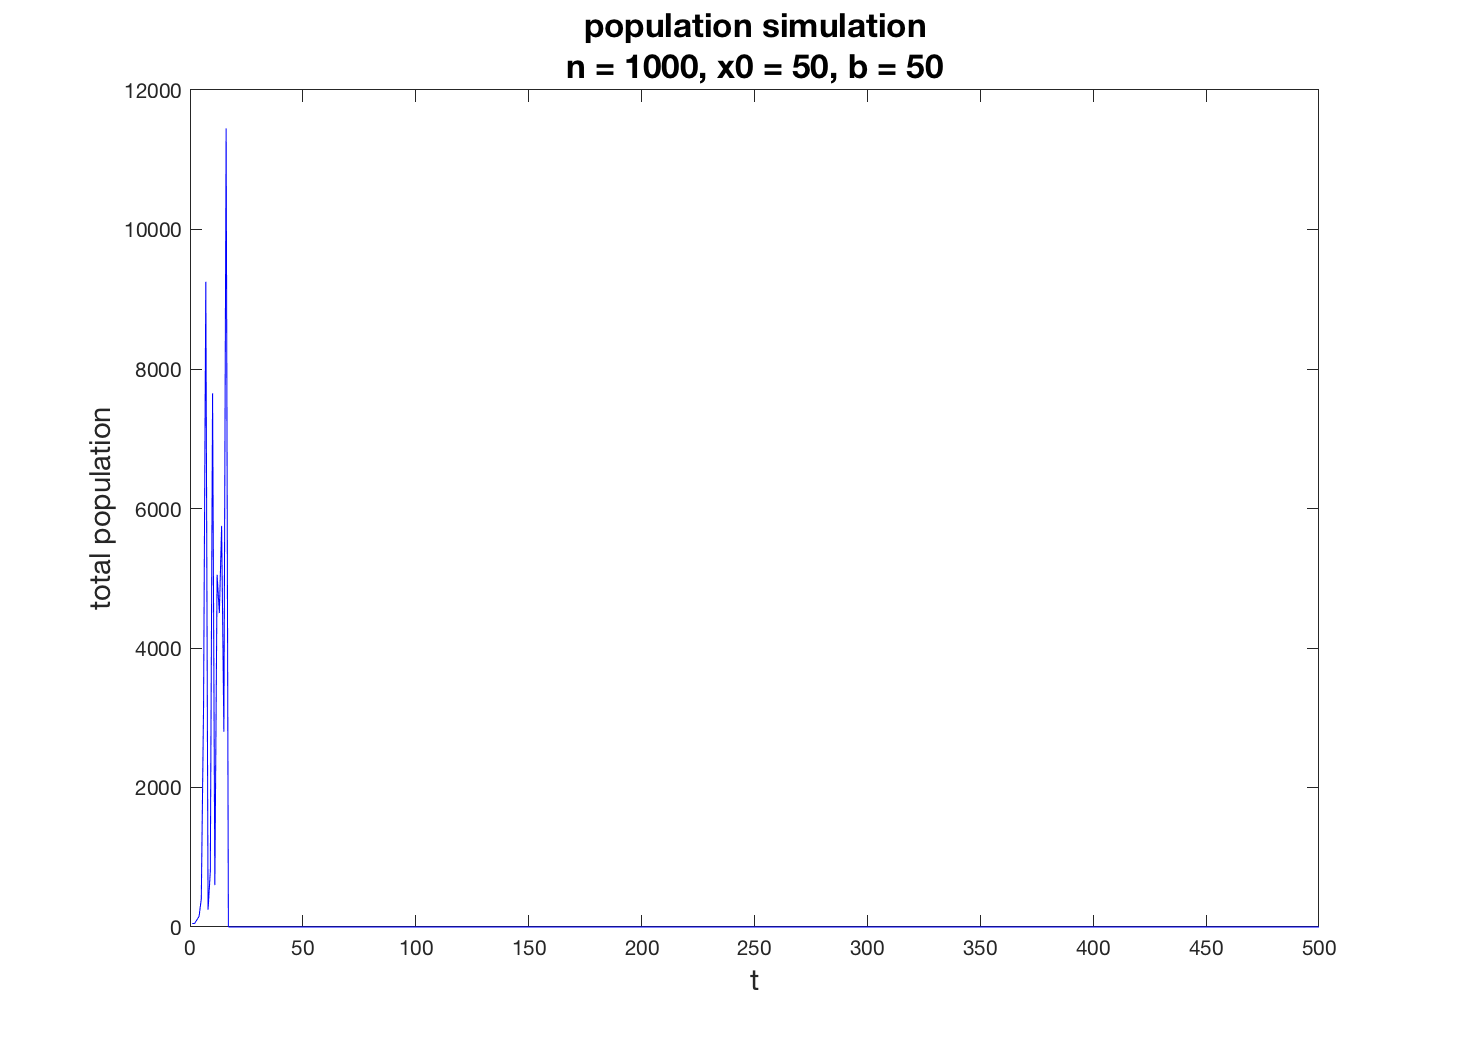
\includegraphics[width = 12 cm, height = 9cm]{single_run n1000 x050 b50.png}
\caption{initial population of 50 and b = 50, in the beginning reproduce but quickly dies}
\label{fig:p1s3}
\end{figure}

\begin{figure}[H] %figure4 x0 = 100 b = 20
\centering
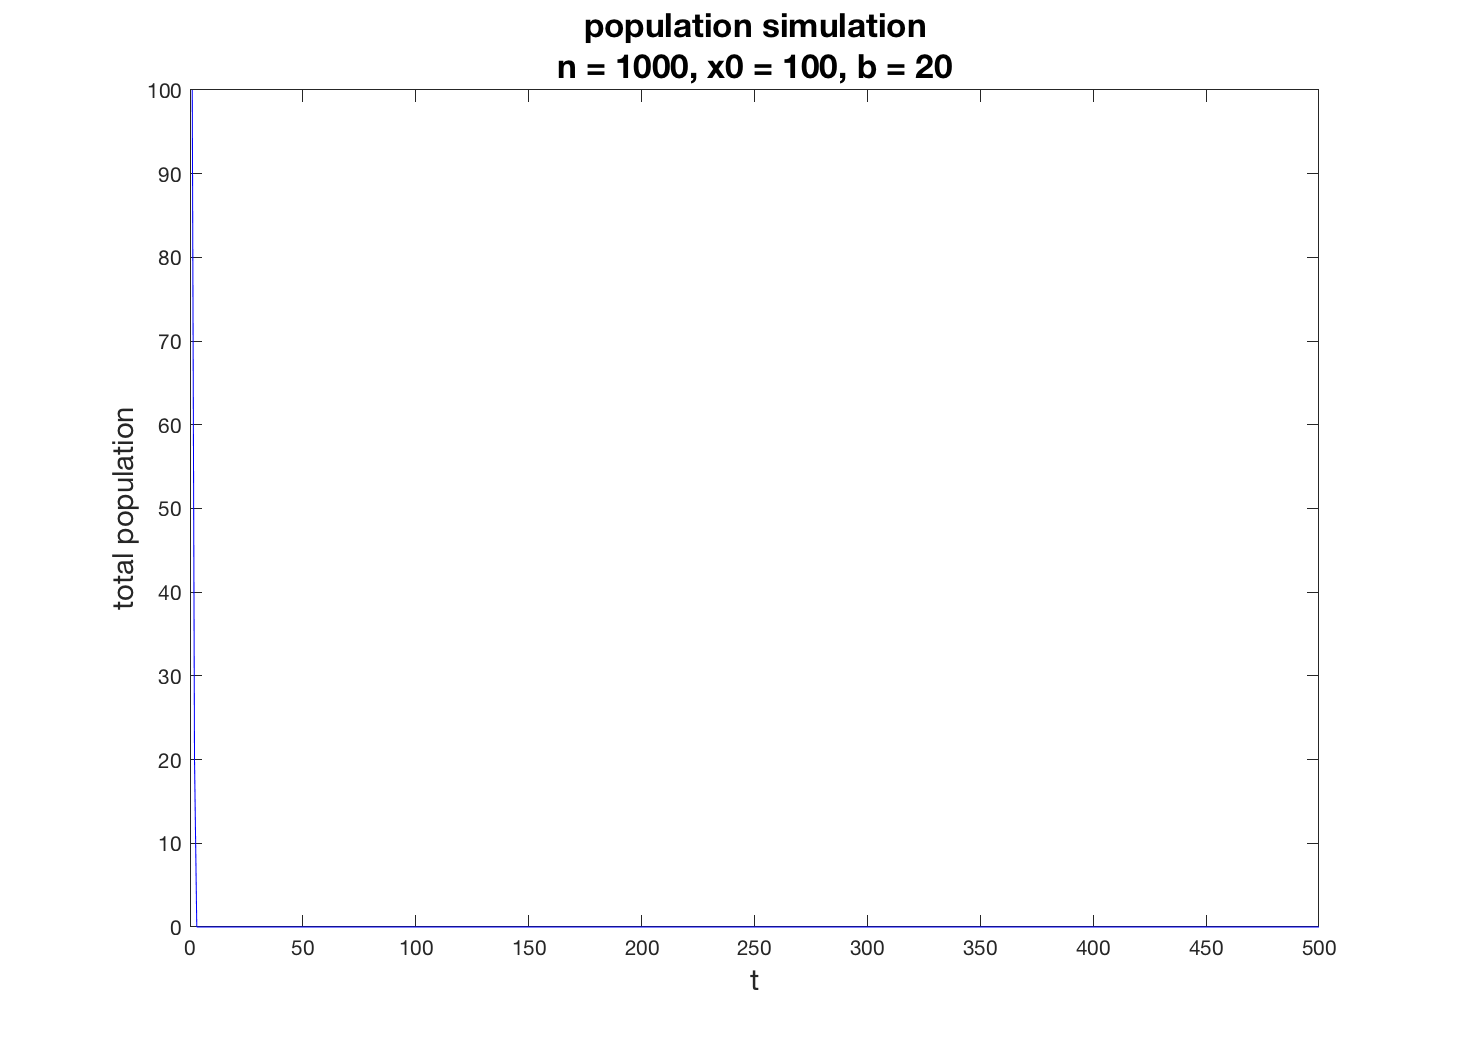
\includegraphics[width = 12 cm, height = 9cm]{single_run n1000 x0100 b20.png}
\caption{initial population of 100 and b = 20, it dies}
\label{fig:p1s4}
\end{figure}

\begin{figure}[H] %figure5 x0 = 100 b = 50
\centering
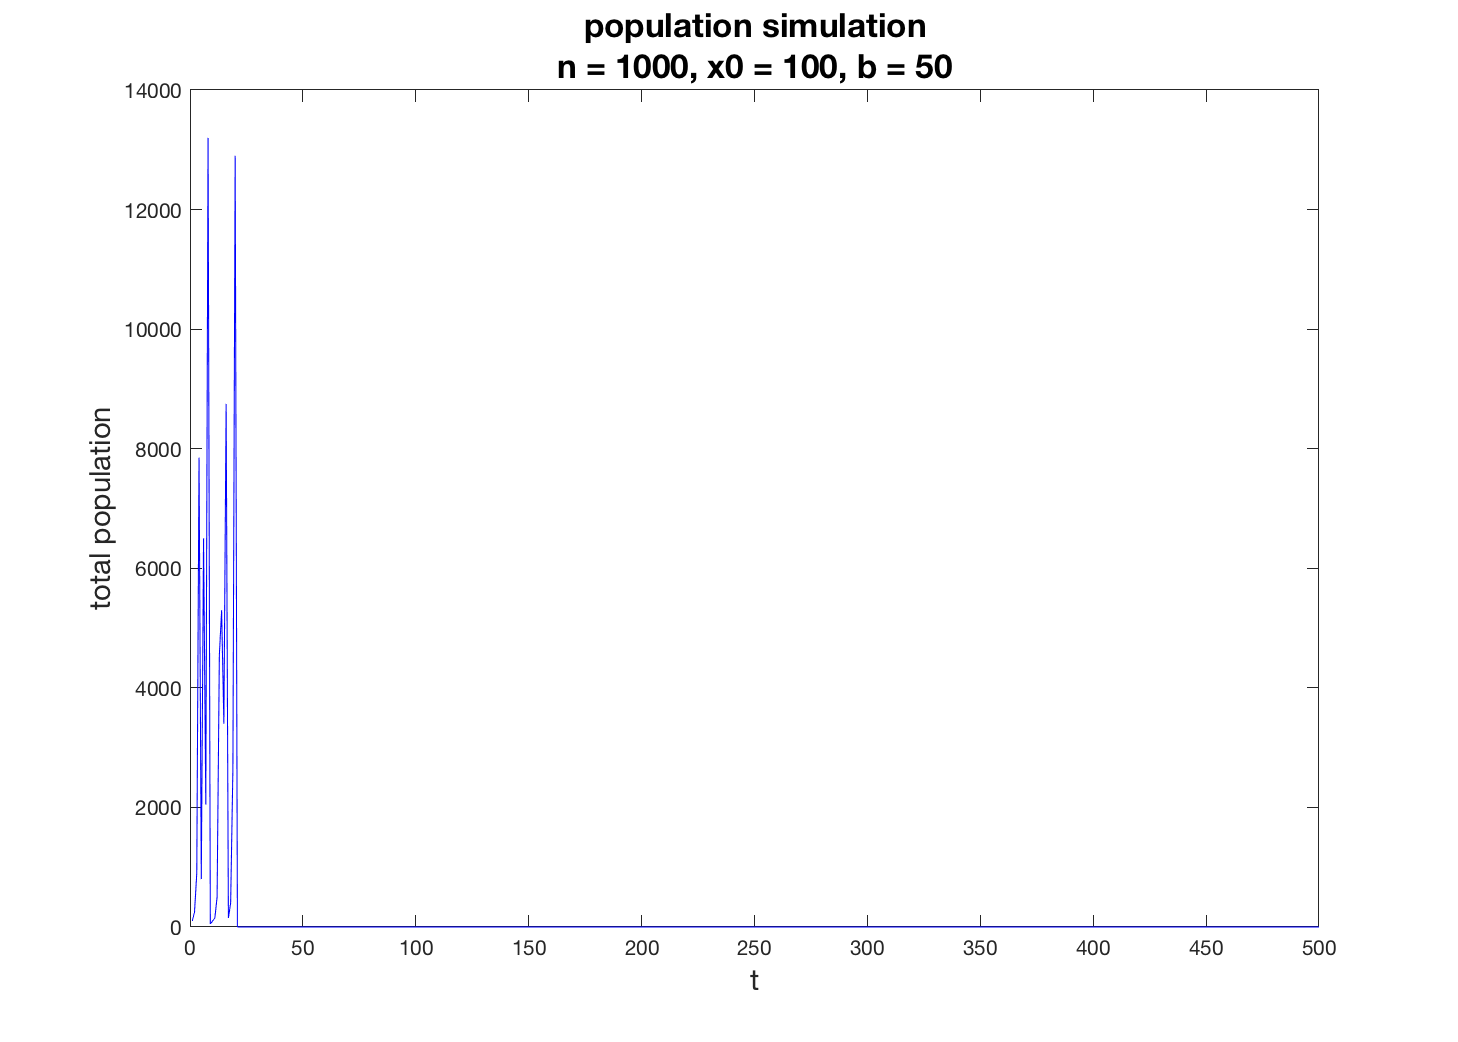
\includegraphics[width = 12 cm, height = 9cm]{single_run n1000 x0100 b50.png}
\caption{initial population of 100 and b = 50, it reproduce in the beginning but quickly dies}
\label{fig:p1s5}
\end{figure}

\begin{figure}[H] %figure 6 x0 1000 b = 10
\centering
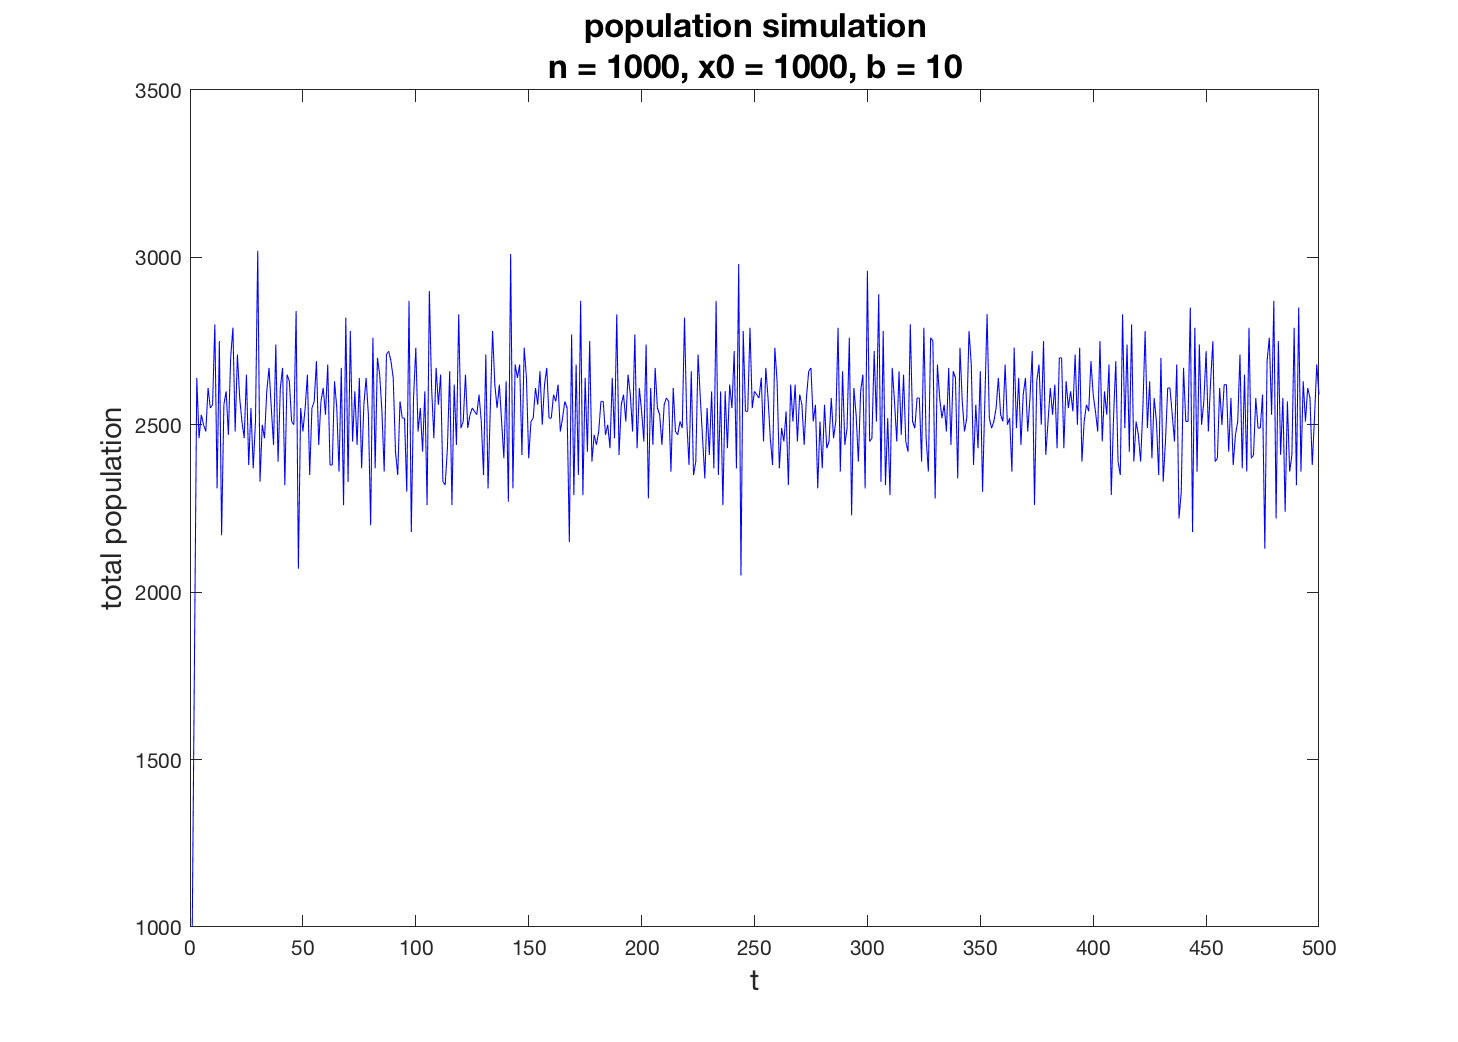
\includegraphics[width = 12 cm, height = 9cm]{single_run n1000 x01000 b10.png}
\caption{initial population of 1000 and b = 10, it show that the population oscillates around 2500}
\label{fig:p1s6}
\end{figure}

\begin{figure}[H] %figure 7 x0 1000 b =20
\centering
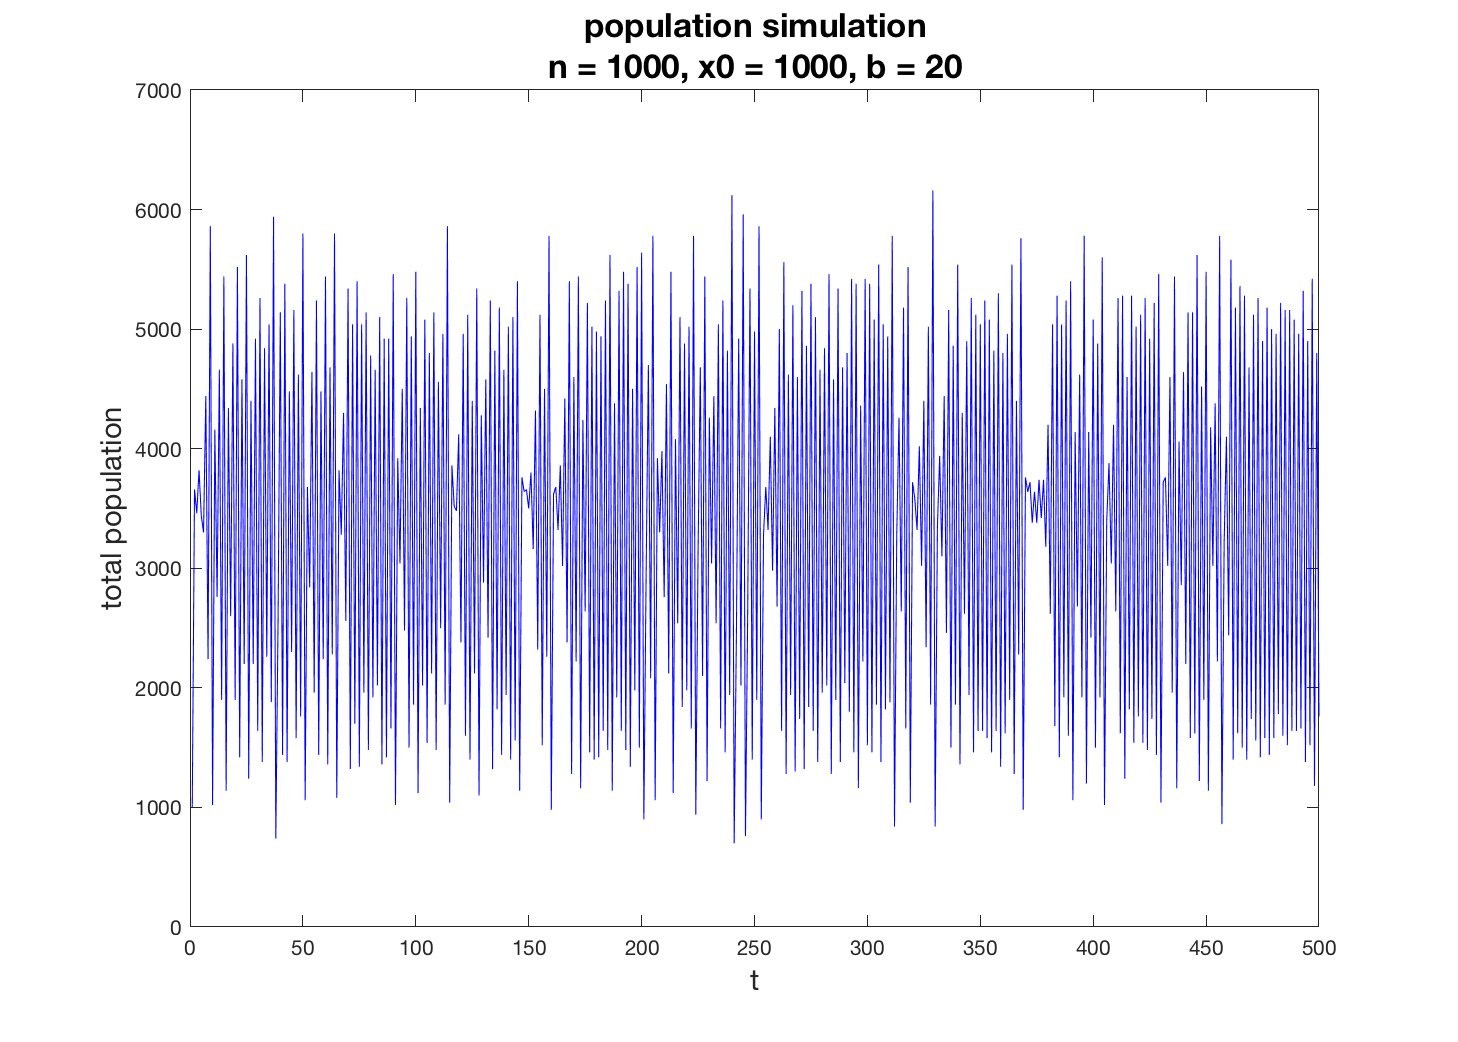
\includegraphics[width = 12 cm, height = 9cm]{single_run n1000 x01000 b20.png}
\caption{initial population of 1000 and b = 20, the populations starts to get chaotic}
\label{fig:p1s7}
\end{figure}

\begin{figure}[H] %figure 8 x0 1000 b =50
\centering
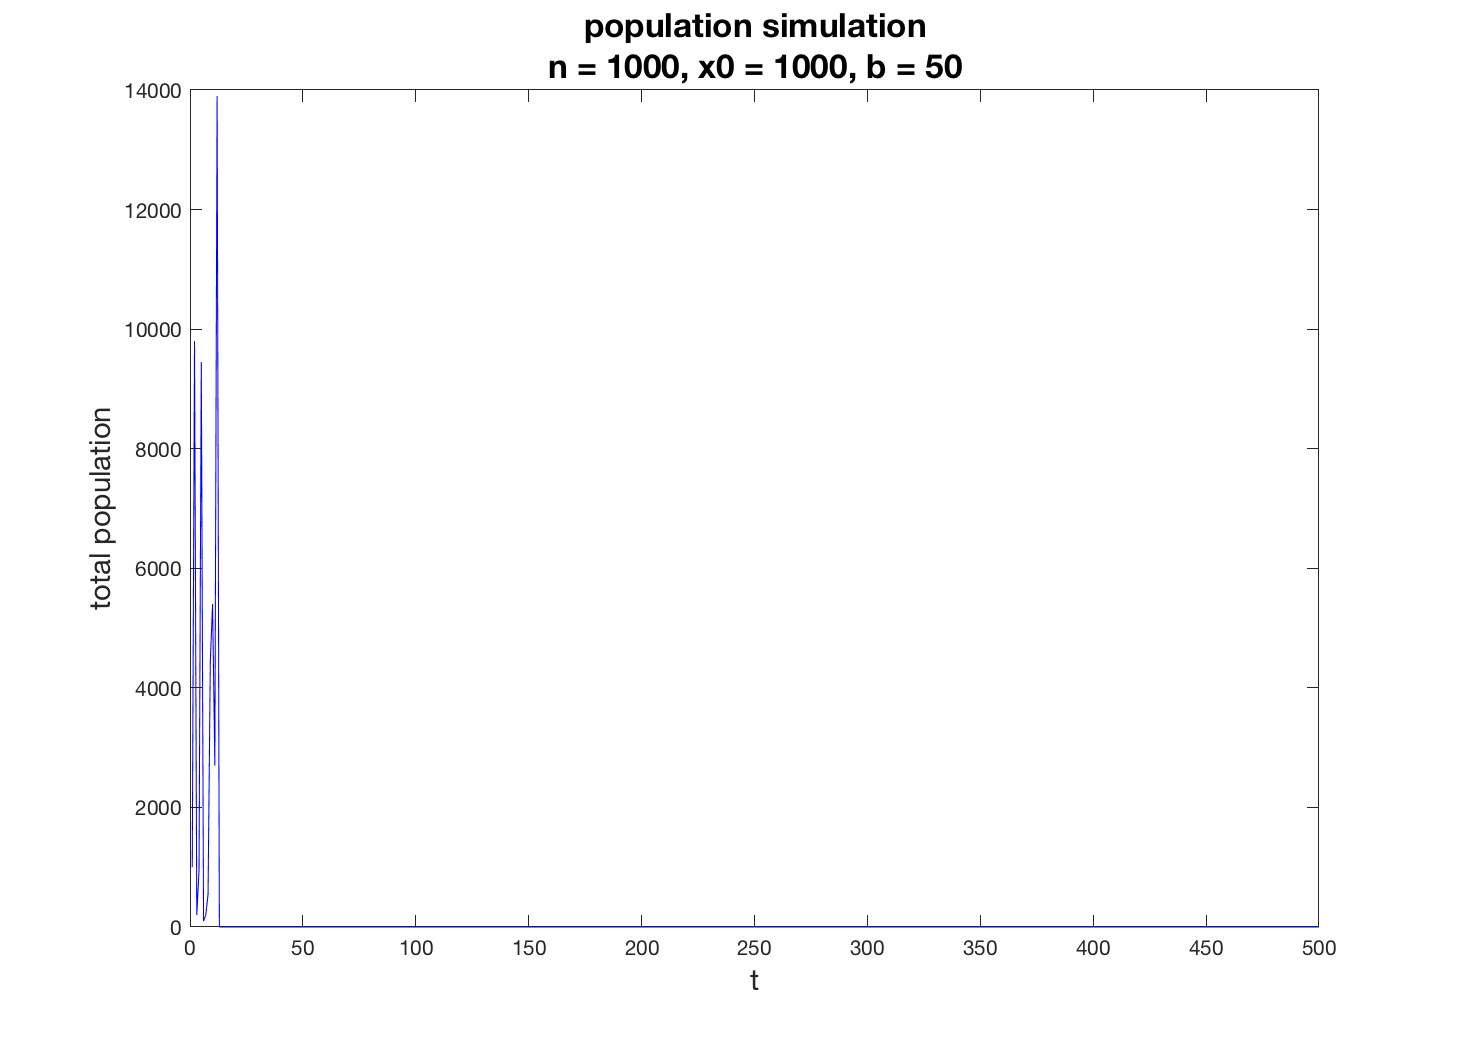
\includegraphics[width = 12 cm, height = 9cm]{single_run n1000 x01000 b50.png}
\caption{initial population of 1000 and b = 500, the populations dies very quick}
\label{fig:p1s8}
\end{figure}


To further study this model, we run it with $A_{0} = 1000$, n= 1000, b = 1, 2, 3, 4, 5,...,48, 49, 50. and at each b value, run the simulation 100 times and plot a phase transition diagram. and we can see that when b = 5-15, the population increases steady and oscillates around a number. When $15<b<35$, the population will get more chaotic and at one time a lot of sites are reproducing, and then the next time steps, they dies because of overcrowding. When $b>35$ the population will dies very quick due to overcrowding. 


\begin{figure}[H] %figure 9 phase transition diagram
\centering
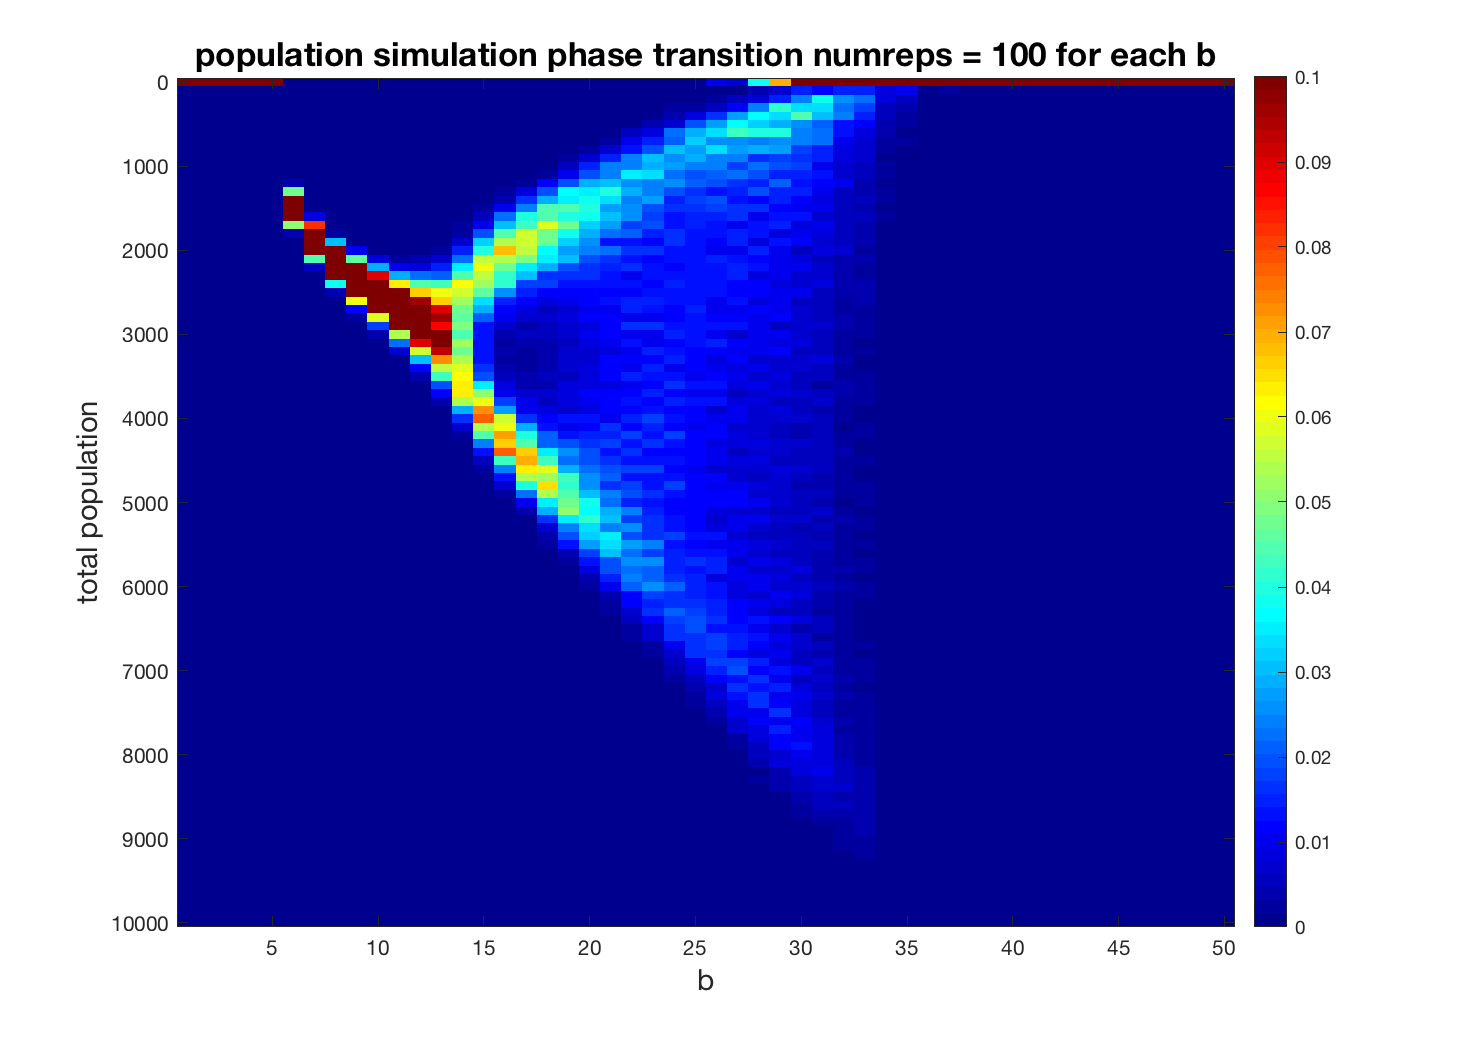
\includegraphics[width = 16 cm, height = 13cm]{q1_phase_r100.png}
\caption{initial population of 1000 and b = 500, the populations dies very quick}
\label{fig:p1q1pd}
\end{figure}

\newpage
\subsection{Mean field model}
We assume the sites are independent and number of individuals at sites is poisson distributed. 
I plot selected mean-field model here for b = 5, 10, 15, 20, 35, 50. The model are after the plot

\begin{figure}[H] %figure 10 mean field model
\centering
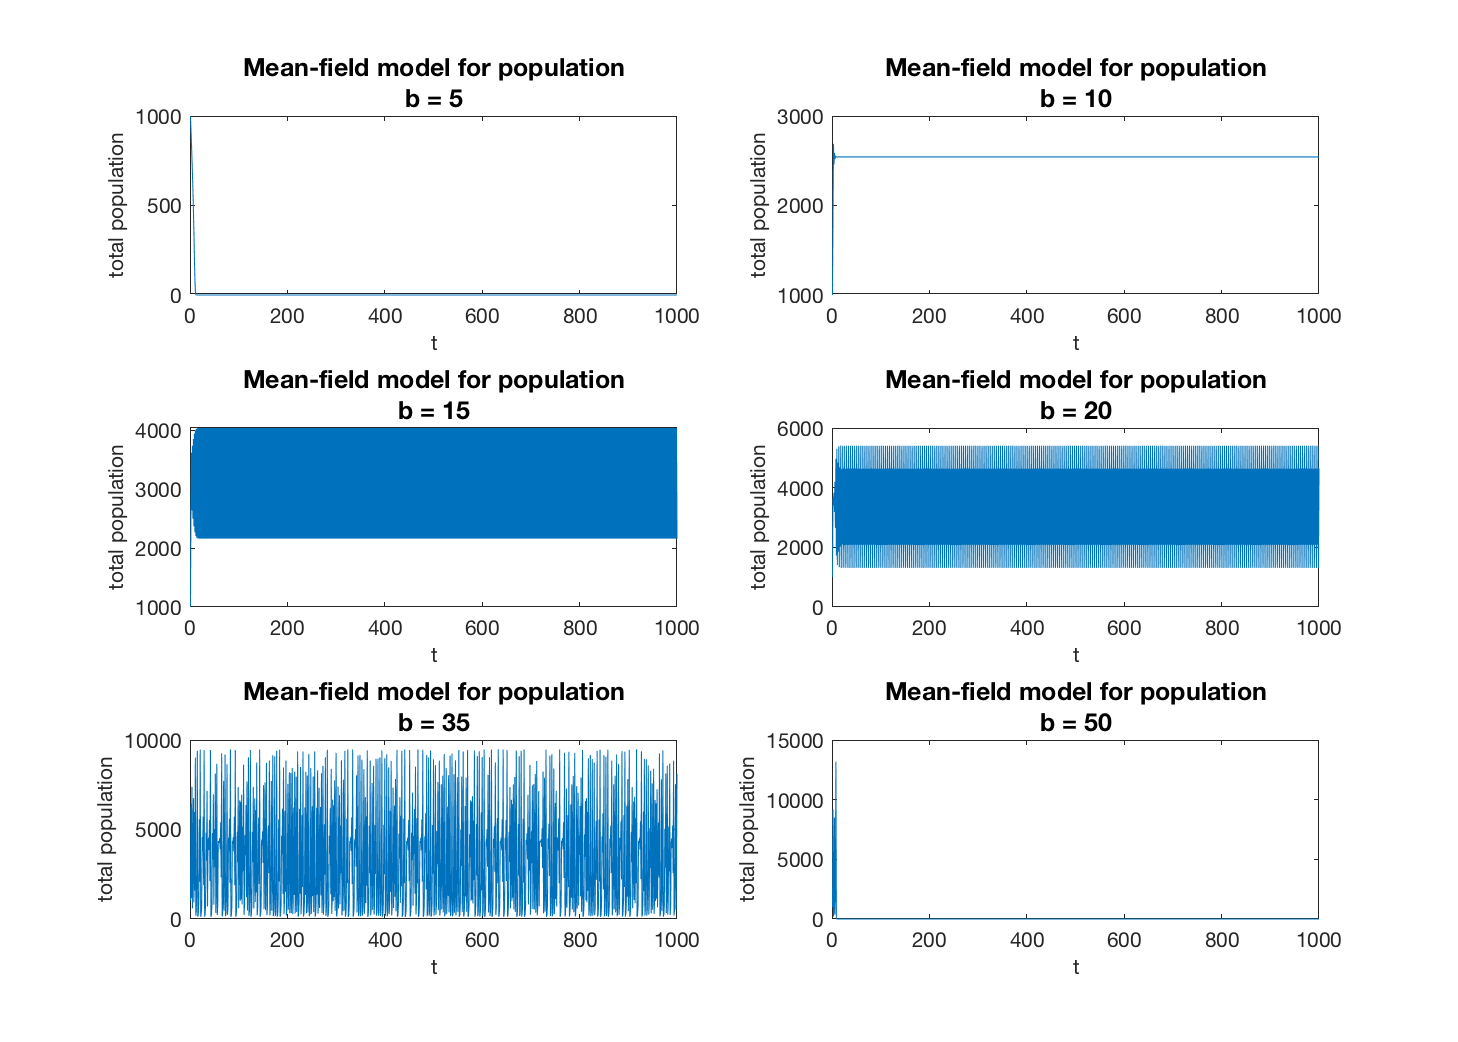
\includegraphics[width = 18 cm, height = 14cm]{meanfield_model.png}
\caption{mean field model with selected b value}
\label{fig:p1q1mf}
\end{figure}

\begin{numcases}{}
	E(A_{t+1}|A_{t}) = n \times \sum_{k=0}^{n} P_{k} \times \phi_{k} \\
	\phi_{k} = \begin{cases}
		b, if k =2\\
		0, if k \neq 2
	\end{cases}
\end{numcases}



following the mean field model, and the population only reproduce if there are exactly 2 individuals at same site, we can write the following:

\begin{equation}
	A_{t+1} = n \times P(2 at site, A_{t}) \times b\\
\end{equation}

\begin{equation}
	A_{t+1} = n \times \frac{(\frac{A_{t}}{n})^{2} \times e^{-\frac{A_{t}}{n}}} {2} \times b
\end{equation}

For steady state, we have $A_{t+1} = A_{t}$.\\

\begin{equation}
	A_{t} = n \times \frac{(\frac{A_{t}}{n})^{2} \times e^{-\frac{A_{t}}{n}}} {2} \times b
\end{equation}

When $A_{t} = 0$, left hand side always equal to right hand side, they are both 0. When $A_{t}  \neq 0$, we have

\begin{equation} \label{eq1}
	1 = \frac{b \times A_{t}}{2n} \times e^{-\frac{A_{t}}{n}}
\end{equation}

Let's rearrange equation (6) and let $\frac{A_{t}}{n} = x $, we have:

\begin{equation}
	1 = \frac{b}{2} \times x \times e^{-x}
\end{equation}

\begin{equation}
	x \times e^{-x} = \frac{b}{2}
\end{equation}

To find the conditions in terms of b for the existence of two further non-zero steady states, we need to find that $f1(x) = x \times e^{-x}$  has intersection with a horizontal line. b need to fulfill the condition that $\frac{2}{b} < 0.3679$, therefore we get: $b > 5.4366$, as b needs to be integer, we get $b > 5$. 


\begin{figure}[H] %figure 11 plot of function
\centering
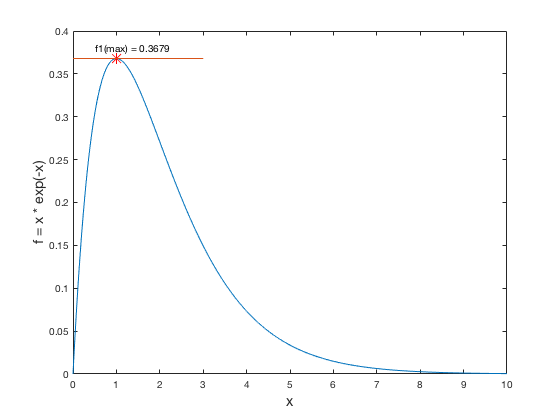
\includegraphics[width = 16 cm, height = 13cm]{q1_2plotfunction.png}
\caption{plot of f1(x) = x * exp(-x)}
\label{fig:p1q1plotfun}
\end{figure}


\newpage
\subsection{Lyapunov exponent}

From the previous section, we have derived the equation for $A_{t}$. that we have 
\begin{equation}
	f(A_t) = n \times \frac{(\frac{A_{t}}{n})^{2} \times e^{-\frac{A_{t}}{n}}} {2} \times b
\end{equation}

\begin{equation}
	f(a) = \frac{b}{2n} \times a^{2} \times e^{-\frac{a}{n}}
\end{equation}

\begin{equation}
	f'(a) = \frac{b}{2n} \times (2a \times e^{-\frac{a}{n}} + a^{2} \times e^{-\frac{a}{n}} \times(- \frac{1}{n}))
\end{equation}

\begin{equation}
	f'(a) = \frac{b}{2n} \times (2a \times e^{-\frac{a}{n}} - \frac{a^{2}}{n} \times e^{-\frac{a}{n}} )
\end{equation}

\begin{equation}
	|\Delta a_{n}| = |\Delta a_{0}| e^{\lambda n}
\end{equation}

to compute Lyapunov exponent $\lambda$ numerically, we use the following:
\begin{equation}
	\lambda = \frac{1}{n} \sum_{t=0}^{n-1} ln |f'(a_{t})|
\end{equation}

The Lyapunov exponent are plotted below: we can see that when $\lambda > 0$ the diverges, that's when b is between 21-30, the population become chaotic. When $b \leq 5$ and $b \geq 31$ $\lambda$ is -infinity that means the system converge very fast, and this explains why the population become extinct very fast for large b. 

\begin{figure}[H] %figure 12 lyaponov exponent
\centering
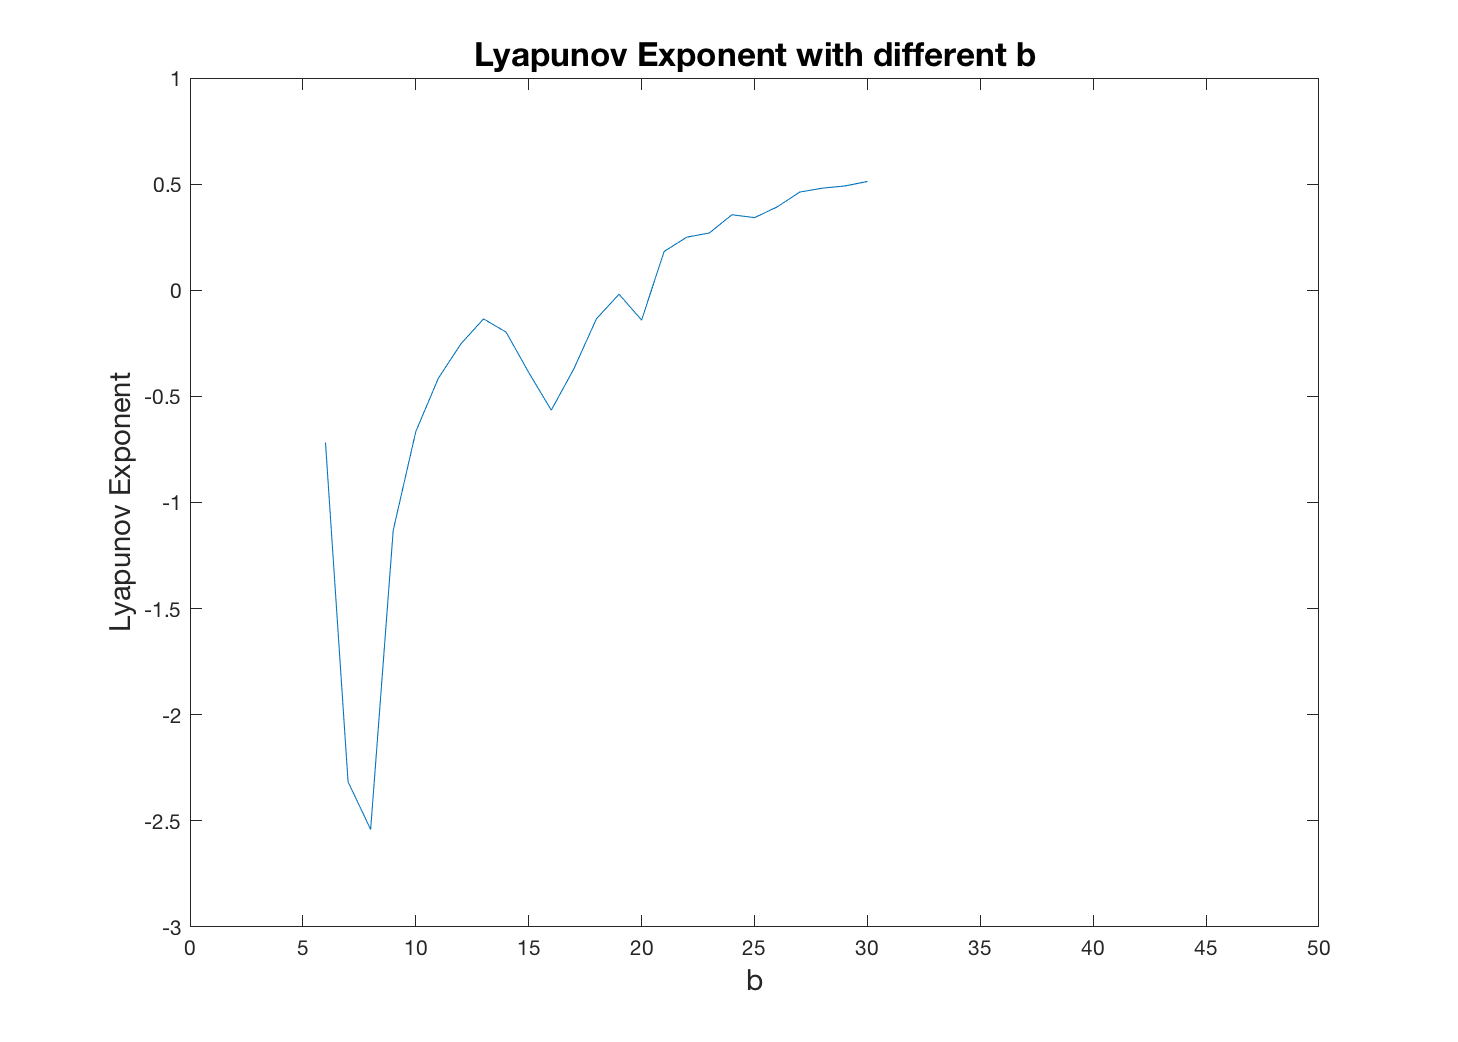
\includegraphics[width = 16 cm, height = 13cm]{lyapunov_exp.png}
\caption{plot of Lyapunov exponent}
\label{fig:p1q1lya}
\end{figure}


%%%%%%%%%%%%%%%%%%%%%%%%%%part 2
%%%%%%%groups of friends

\newpage
\section{Groups of friends}
\doublespacing
In this part, we used a model to simulate how students make friends. Initially, there are N students, and they are all alone in a group contains only one student. At each time step, a group is picked:

\begin{enumerate}
\item If the picked group contains only one student, this students will join a group with size k with probability of k/N.  
\item if the picked group size i ($i > 1$), then this group will split up with probability of ri. 
\end{enumerate}


\subsection{simulations in Matlab}
First, we simulate the above model with 100 students, r = 0.01 and 100 replications. First, we plot the group size vs frequence on a log log scale. Second, we get the relative frequency with group size histogram taken on a log scale that is we take groups size [1,2,4,8,16,32,64,128] and plot the group size vs relative frequency on a log log plot. in figure \ref{fig:loglog1}, we can observe that the group distribution following the power law. 


\begin{figure}[H] %f13 loglog with groupsize 1:1:100
\centering
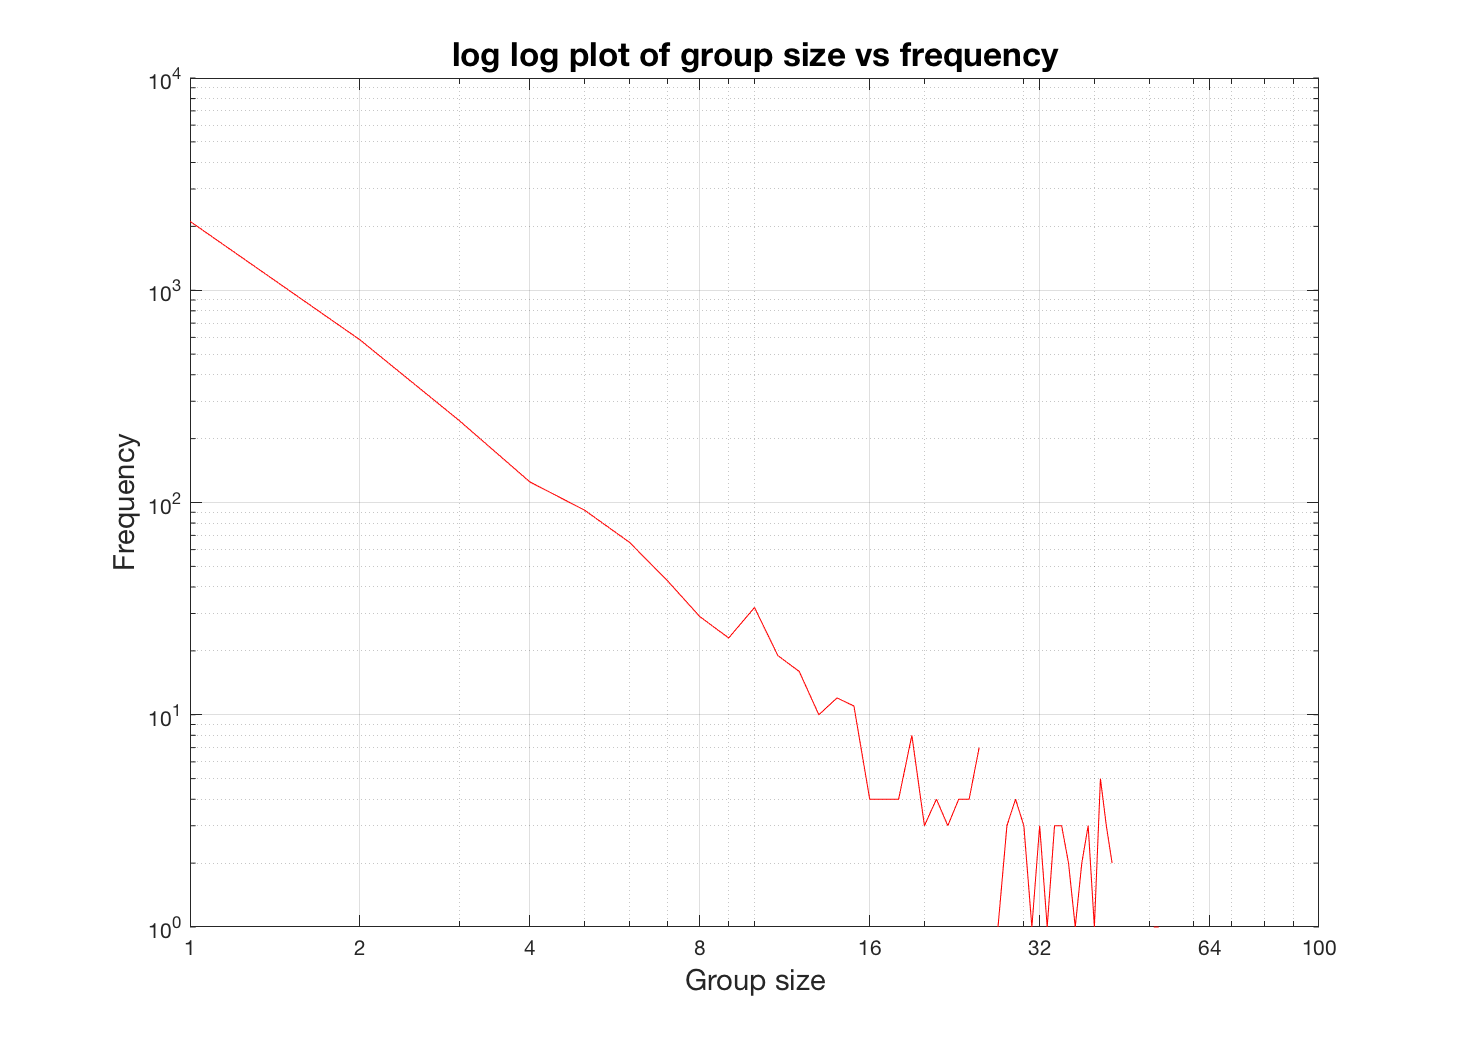
\includegraphics[width = 12 cm, height = 9cm]{loglog2.png}
\caption{log log plot of group size vs frequency}
\label{fig:loglog2}
\end{figure}

\begin{figure}[H] %f14 loglog with groupsize 1 2 4 8 16 32
\centering
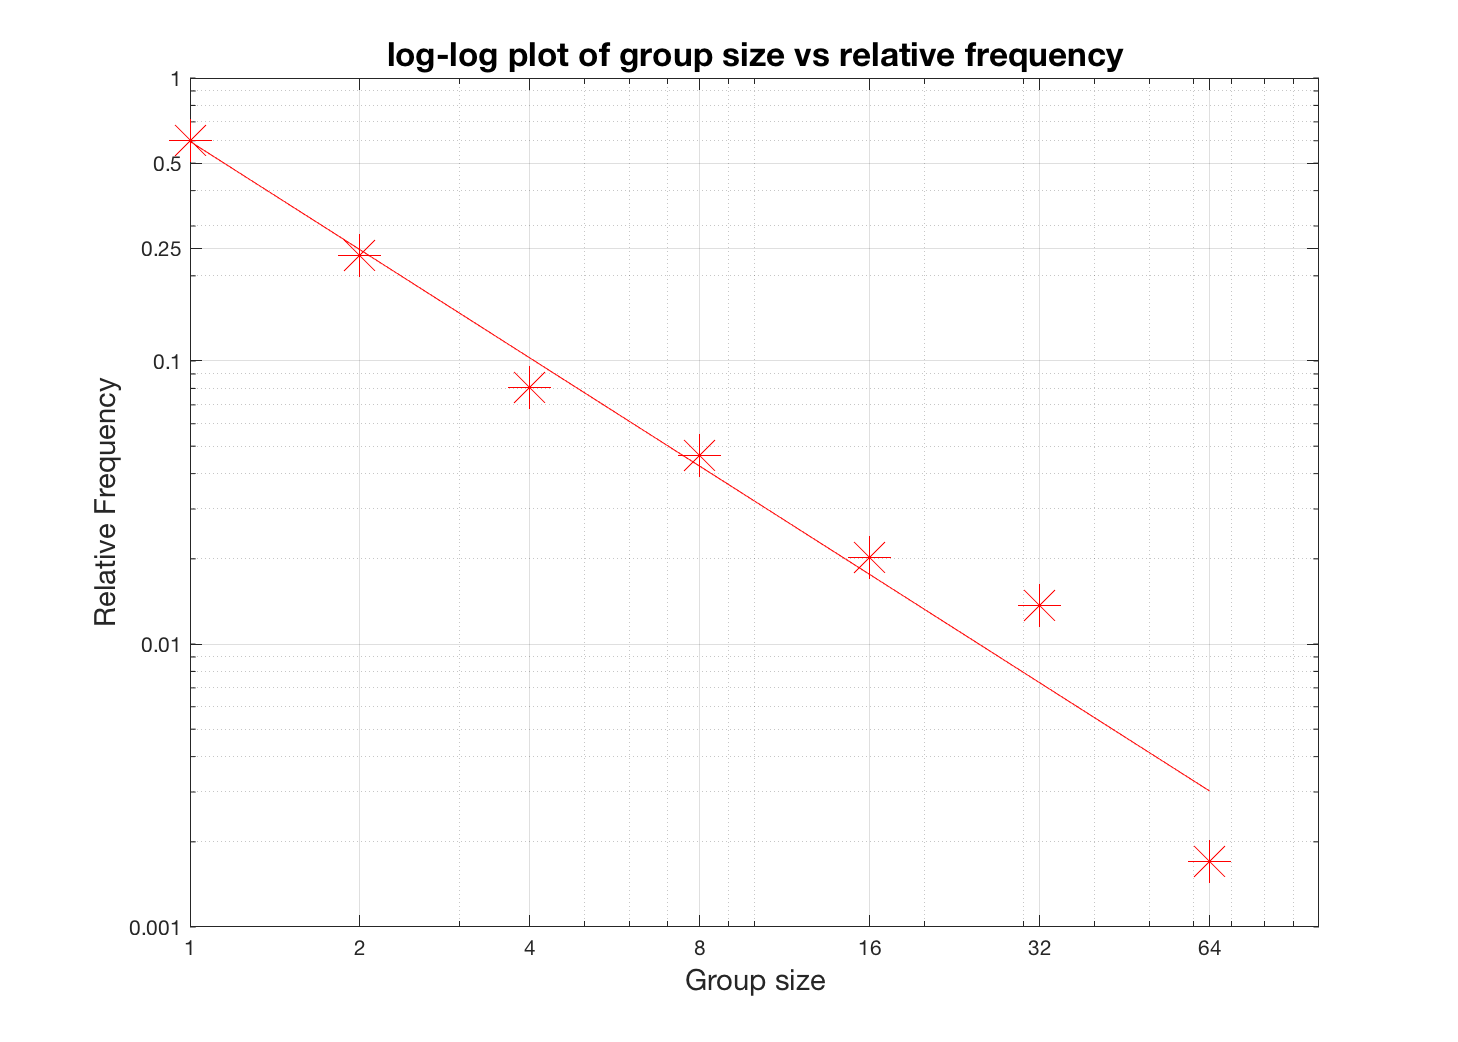
\includegraphics[width = 12 cm, height = 9cm]{loglog1.png}
\caption{log log plot of group size vs relative frequency}
\label{fig:loglog1}
\end{figure}

To investigate the how the group size distribution changes with r, we run the model with r from 0.001:0.001:0.1 with 100 replications. In \ref{fig:loglog3}, I choose some r values to plot shows how the group size changes, and in \ref{fig:loglog4}, the whole group distribution is shown on a 3d plot, it might be a little difficult to from the colourful map, but we can observe the z-axis value that the relative frequency of the group. \par
When r is small at 0.001 we have groups of size 1 and 2 around $\frac{1}{4}$ of the population and some large groups. when we increase the r, then the number of groups of 1 become the dominant group in the distribution and large group appear less and less. With a bigger r, the larger group will split up if it was chosen at time t. For example, setting r = 0.1, it means that groups of size 10 + will slip up at the probability of 1 if chosen at time t. 

\begin{figure}[H] %f15 loglog with r value
\centering
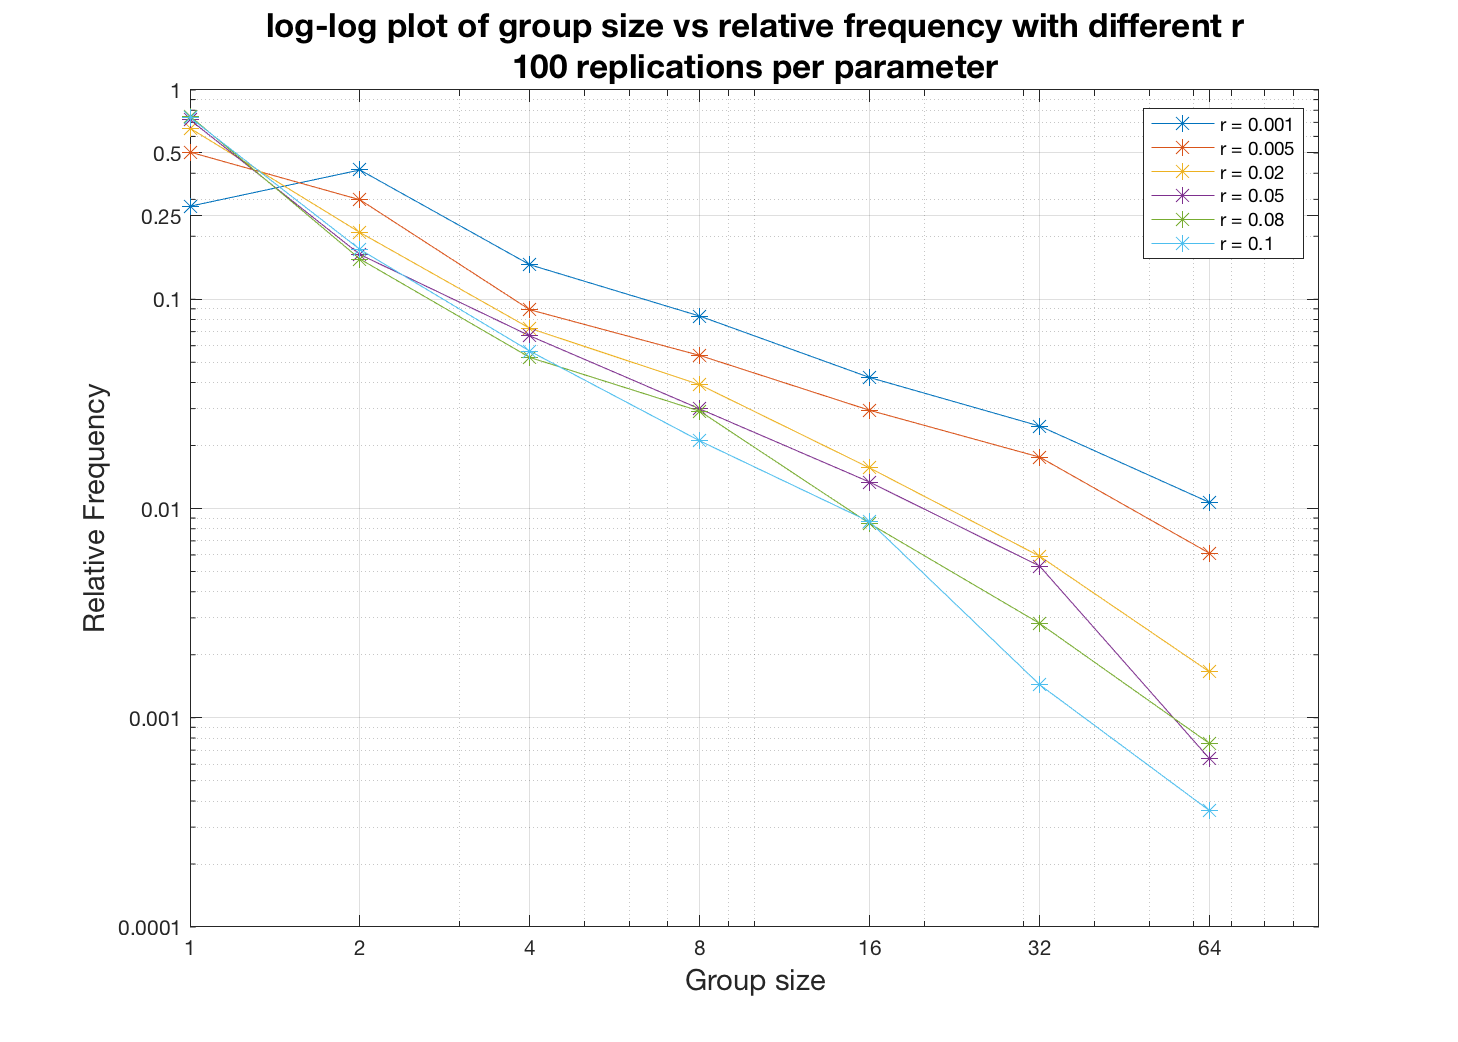
\includegraphics[width = 14 cm, height = 11cm]{logloggr100.png}
\caption{log log plot of group size vs relative frequency with different r}
\label{fig:loglog3}
\end{figure}

\begin{figure}[H] %f15 loglog with r value
\centering
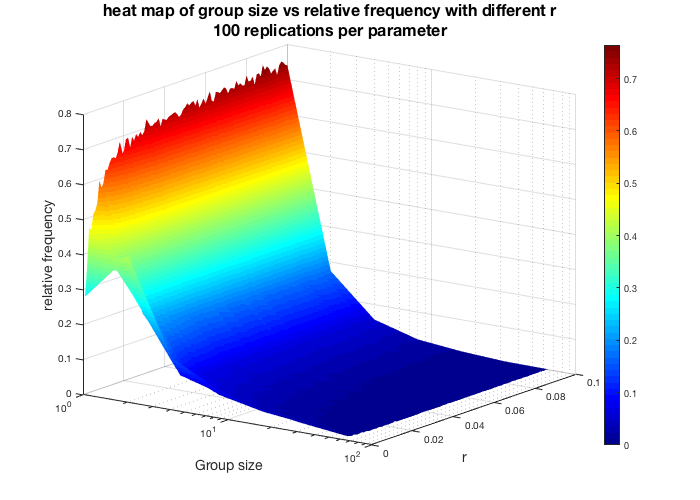
\includegraphics[width = 16 cm, height = 13cm]{hmq2.png}
\caption{the distribution of groups with different r showing on a 3d plot}
\label{fig:loglog4}
\end{figure}





%%%%%%%2.2 master equation
\newpage
\subsection{Master Equation}



%%%%%%%%%%%%
%%%%%%%%%%%%ATTENTION NEEDS HERE IN THIS PART
%%%%%%%%%%%%%%%



%%%%%%%%%%%%%%%%%%%%%%%%%%part 3
%%%%%%%Network Epidemics

\newpage
\section{Network Epidemics}
\doublespacing

\subsection{random undirected social network}

An undirected networking was made with 5000 students and a link density of 0.0016. we use matrix A to represent the network, as the network is undirected, we have A as a symmetric matrix, and with a link density of 0.0016, we generate A and plot the histogram of the degree distribution. The average degree of this network is around 8 and the degree follows a binomial distribution. 

\begin{figure}[H] %f16 frequency of histogram
\centering
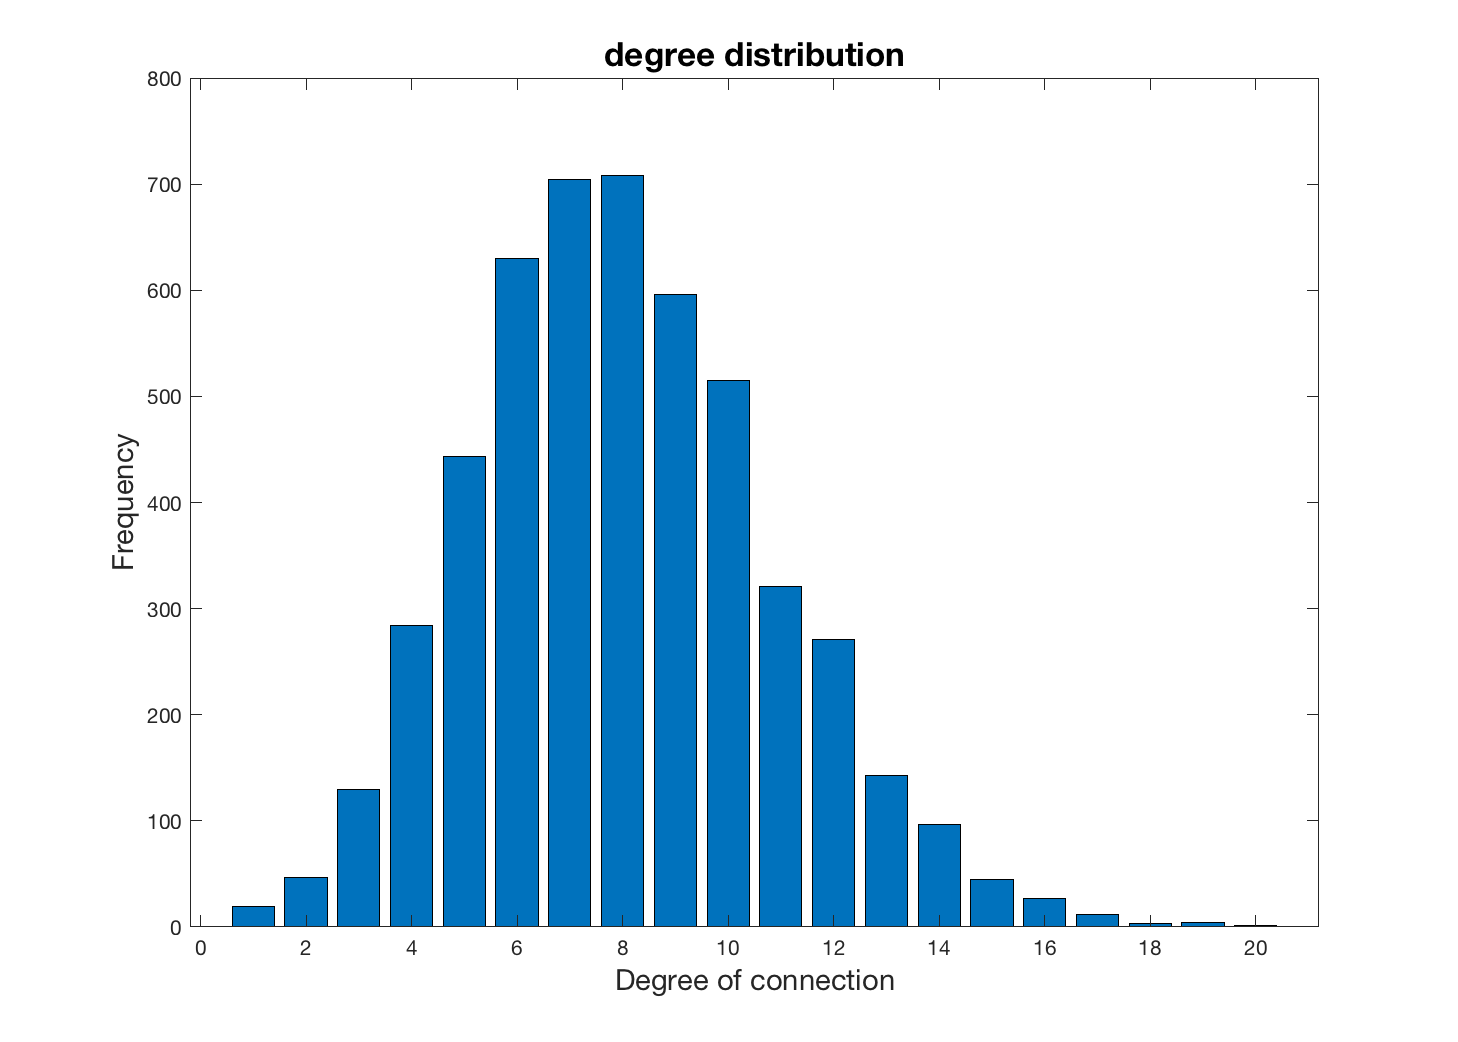
\includegraphics[width = 12 cm, height = 9cm]{randomf.png}
\caption{Frequency of the connection degree}
\label{fig:randomconnect}
\end{figure}

\newpage
\subsection{Infection within the random network}

A infection on above random network was modelled. In the beginning, there are 100 random infected students. The infection will spread according to:

\begin{enumerate}
\item An uninfected student will get infected depends on the infected student he is connected with. $P_{infected}(n) = 1 - e^{-pn}$.  
\item An infected student will recover with the probability of r = 0.03.
\item A recovered student can get infected again. 
\end{enumerate}

To study the model, we set p = 0.01 and plot the number of infected students over time and it showed that the infection spreads very quick. At around 200 time, the total number of infected students are around 3000, and it stays stable around that number, which is more than half of the population. To further investigate, we run the model with p = 0.001:0.001:0.01, and the infection does not spread for $p \leq 0.003$, the infection will stay around the initial number when p = 0.004, and the infection will spread when $p \geq 0.005$, and the larger the p, the faster the spread of the infection and more infected students. \par

Finally, in Figure \ref{fig:infectprp} we can see than the infection will die when $r/p \geq 10$ and spread very fast when $r/p \leq 5$.

\begin{figure}[H] %f17 p0.01
\centering
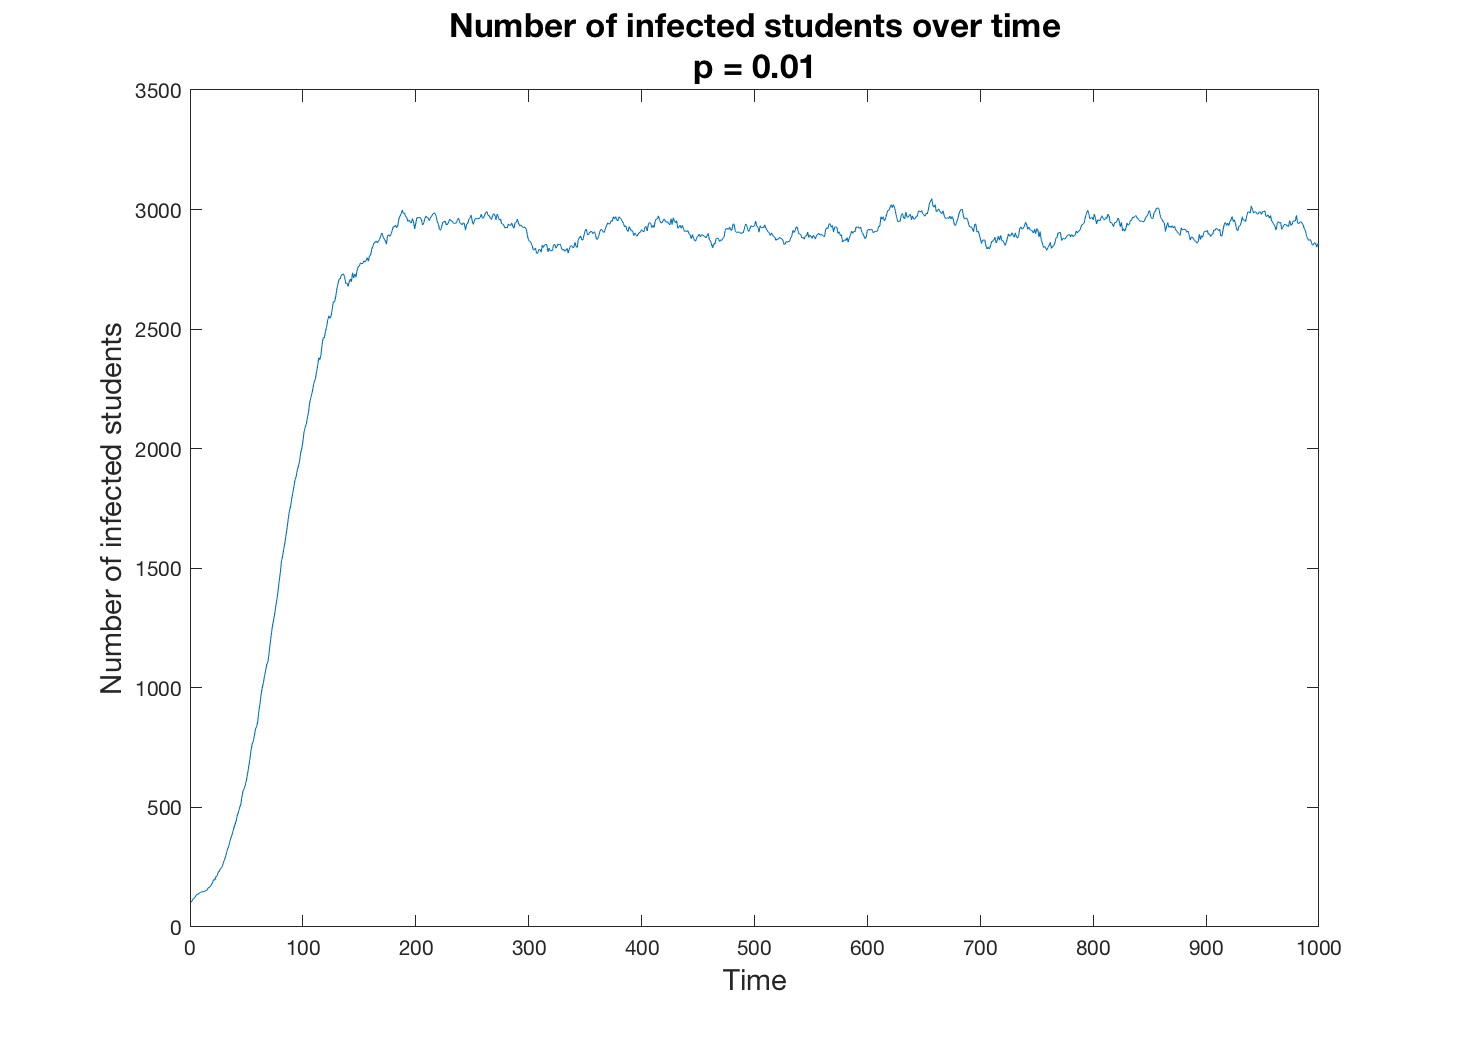
\includegraphics[width = 12 cm, height = 9cm]{infectp001.png}
\caption{Number of infected individuals against time with p = 0.01}
\label{fig:infectp001}
\end{figure}

\begin{figure}[H] %f18  10 runs with different p
\centering
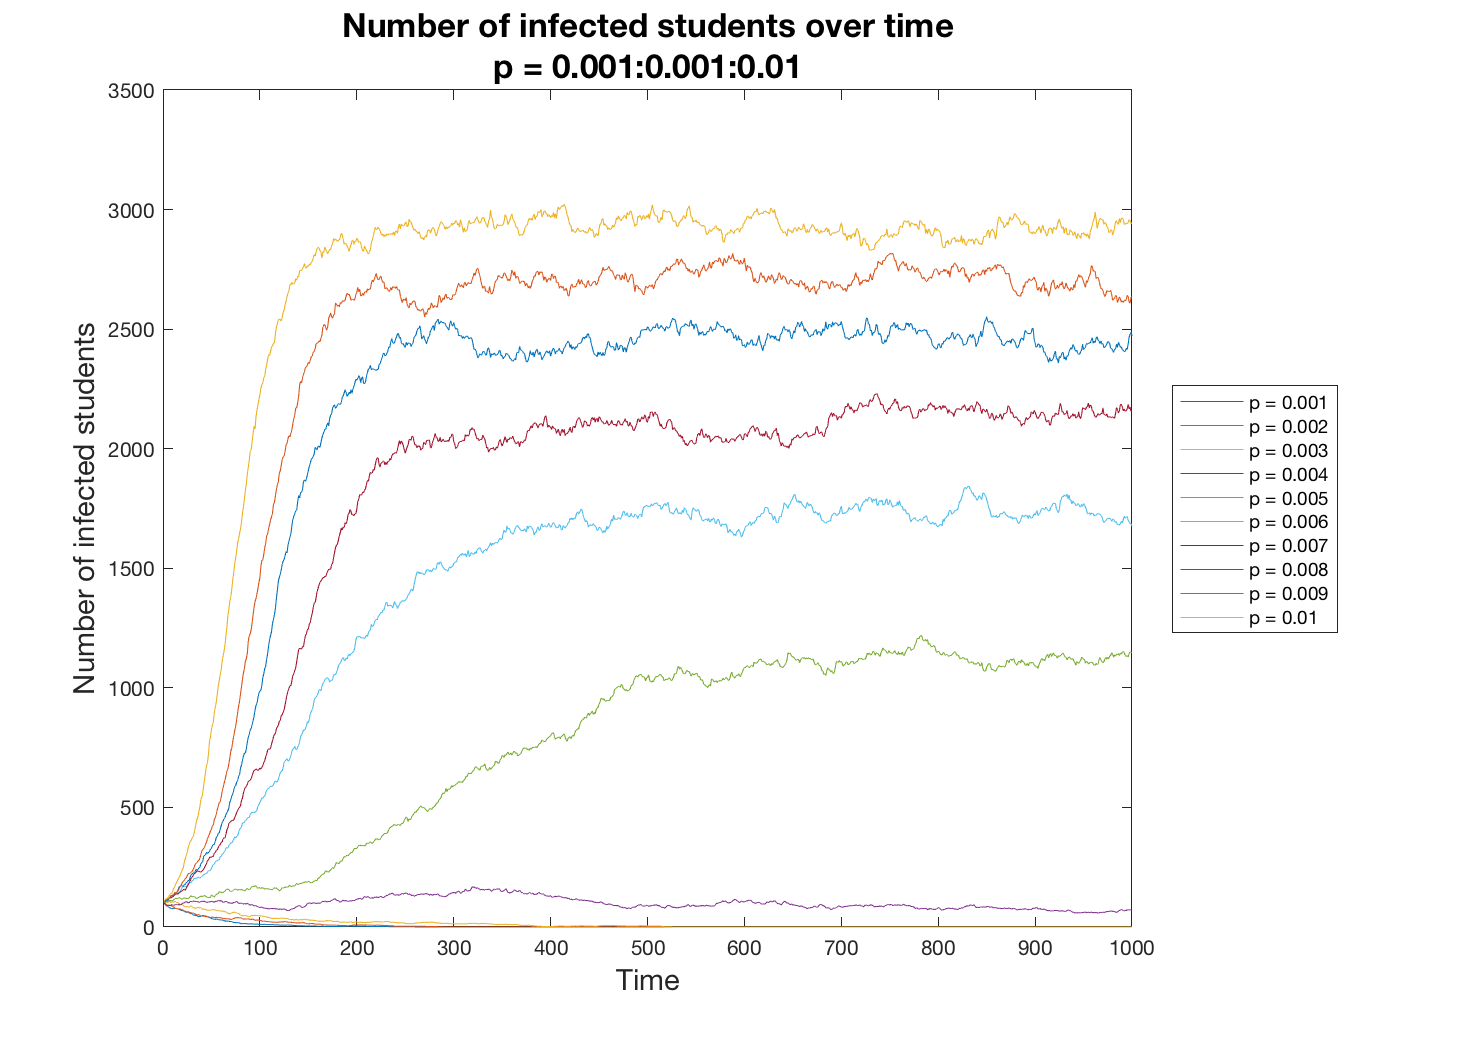
\includegraphics[width = 12 cm, height = 9cm]{infectp10r.png}
\caption{Number of infected individuals against time with different p}
\label{fig:infectp10r}
\end{figure}

\begin{figure}[H] %f19 frequency of histogram
\centering
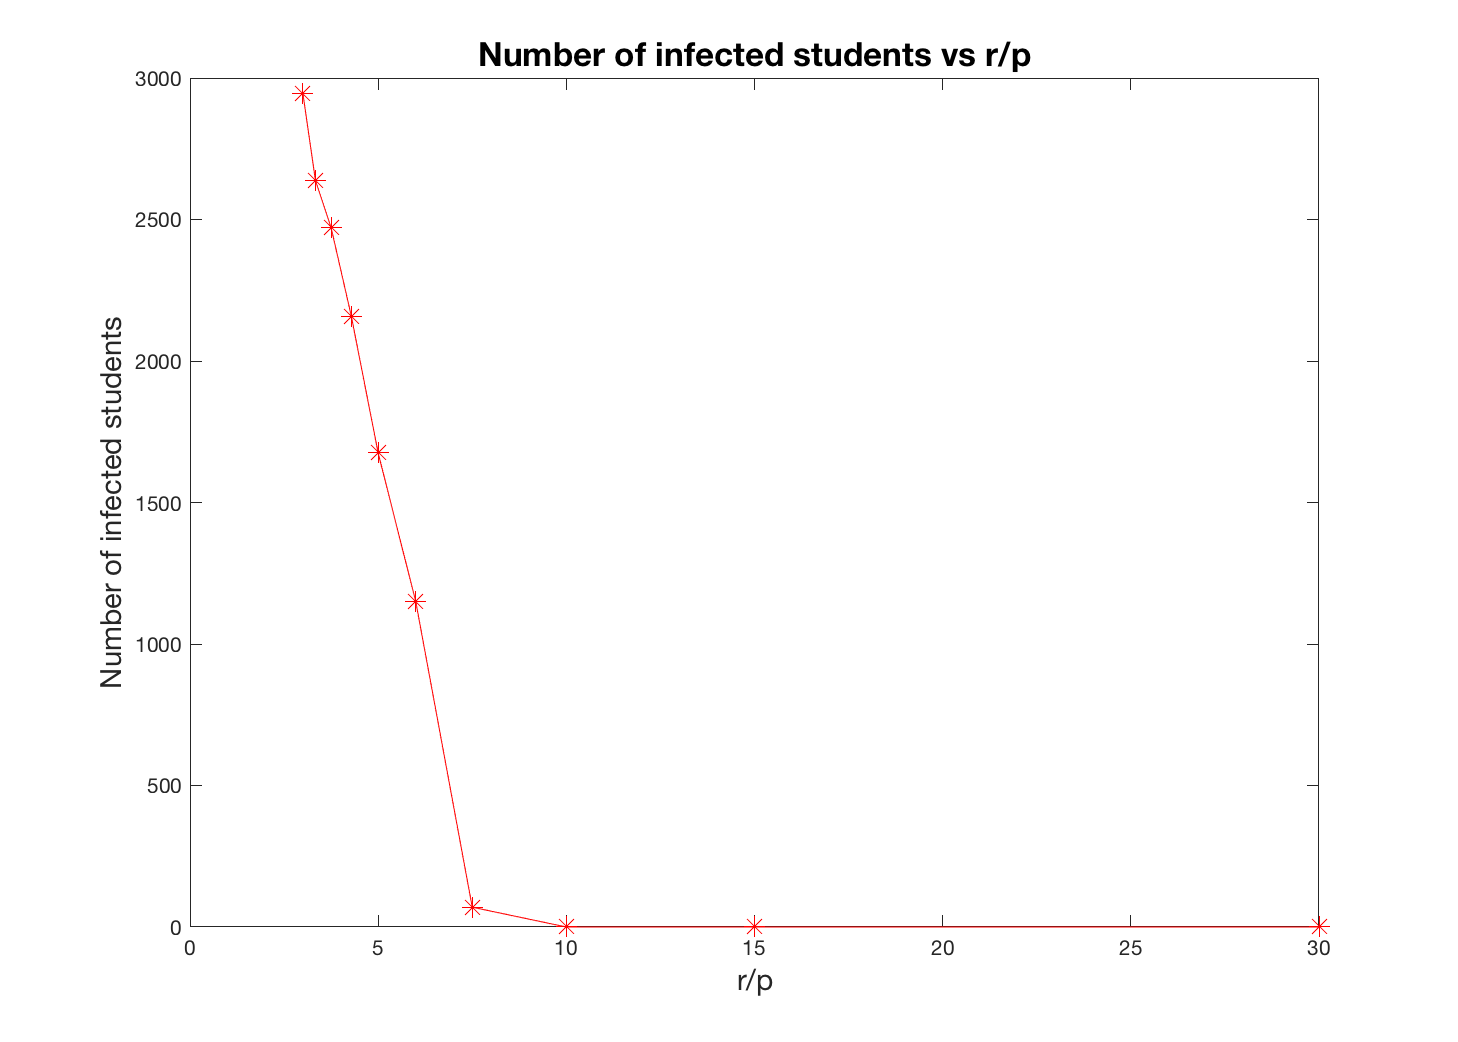
\includegraphics[width = 12 cm, height = 9cm]{infectprp.png}
\caption{Number of infected individuals vs. r/p}
\label{fig:infectprp}
\end{figure}



\newpage
\subsection{Infection within the random network}

In this part, we create a network with preferential attachment, starting at $t_{0}$, there are 2 students that are linked. Each time step, one new student is added to the network and he will chose to connect with a students at $p = \frac{k_{i}}{2(n-2)}$. 

First, we can see that in Figure \ref{fig:degreehist}, the connection degree distribution follows the power law distribution. The average degree of the network is around 2. But to have a better idea, we take histogram at interval of $2^{i}$. And in Figure \ref{fig:degreeloglog}, it eliminates the random noise, and shows a strong power law distribution for the preferential network.

\begin{figure}[H] %loglog plot for degree
\centering
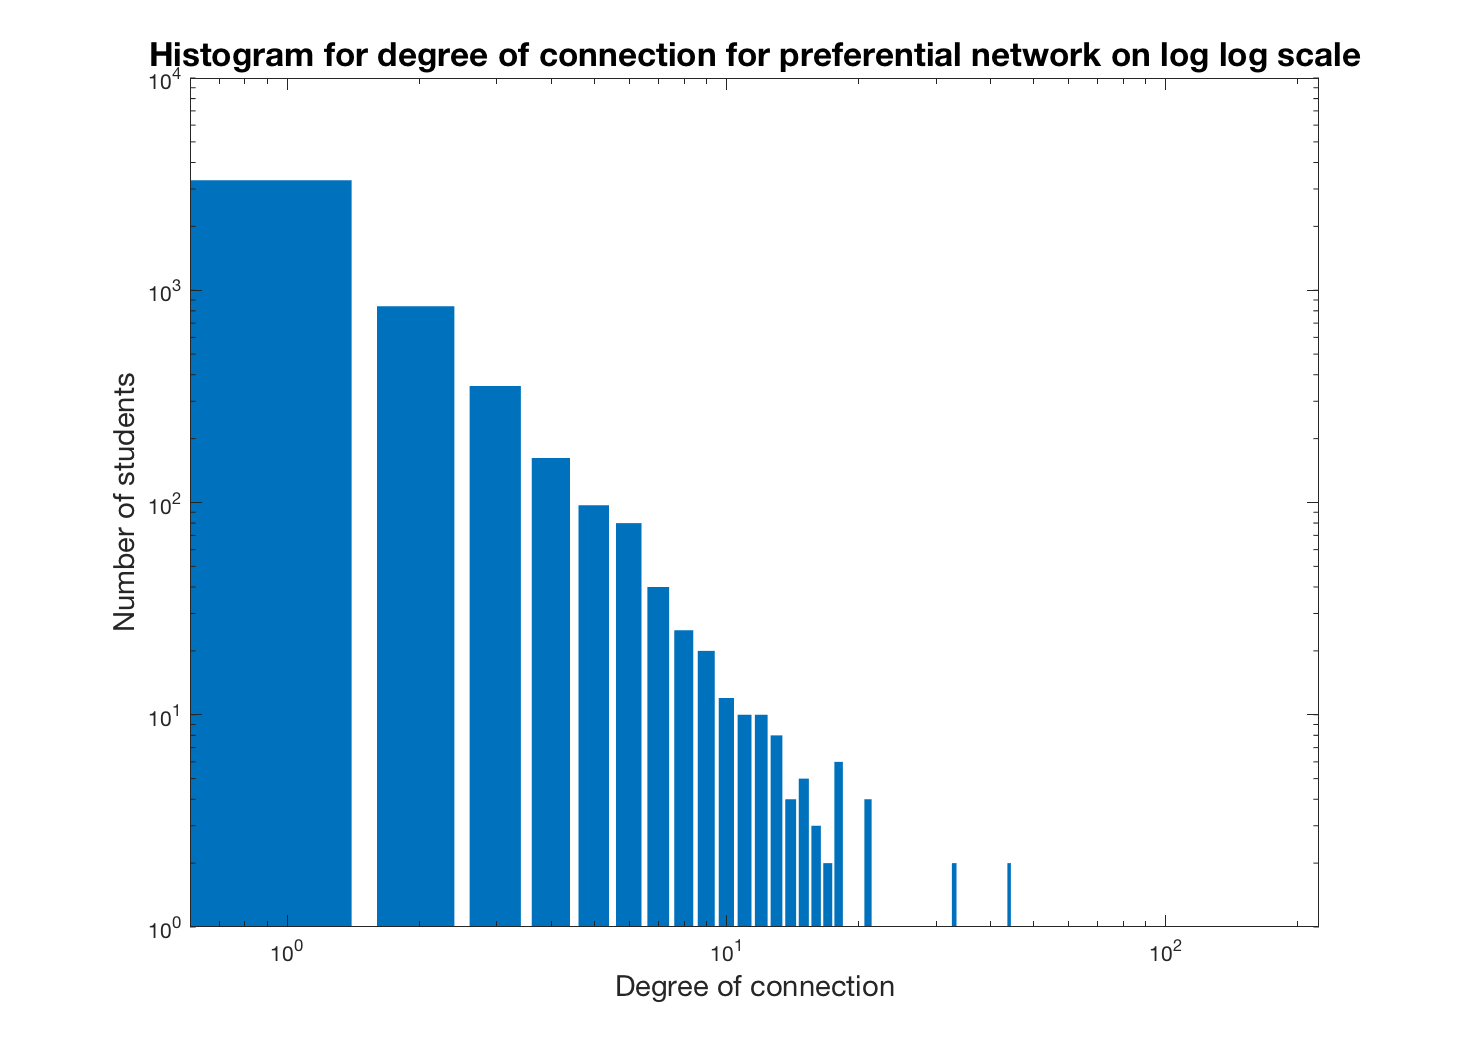
\includegraphics[width = 14 cm, height = 11cm]{p_nw2.png}
\caption{Histogram of the degree distribution }
\label{fig:degreehist}
\end{figure}

\begin{figure}[H] %loglog plot for degree
\centering
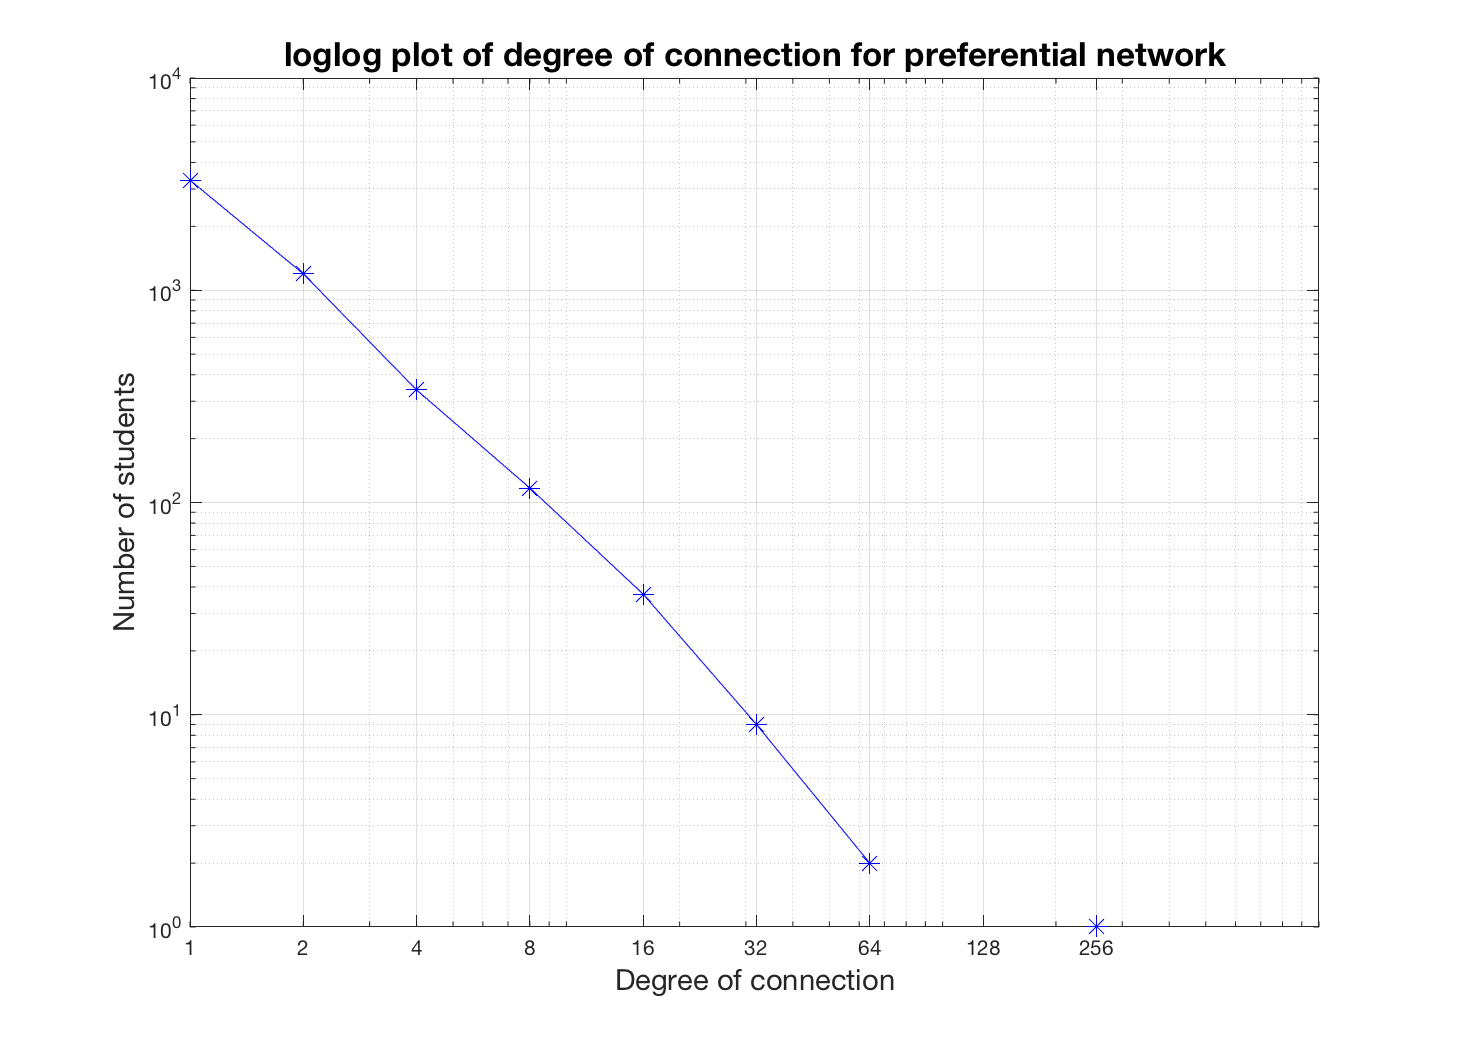
\includegraphics[width = 16 cm, height = 13cm]{p_nw.png}
\caption{loglog plot of degree of connection}
\label{fig:degreeloglog}
\end{figure}


%%%%%%%3.4 master equation
\newpage
\subsection{Master Equation}



%%%%%%%%%%%%
%%%%%%%%%%%%ATTENTION NEEDS HERE IN THIS PART
%%%%%%%%%%%%%%%




%%%%%%%3.5 infection
\newpage
\subsection{infection with the preferential attachment network}

Here, the infection in 3.2 are simulated in the preferential network created in 3.3. We can see in Figure \ref{fig:pnwinf} that the number of infection will die when $p \leq 0.005$, the infected number will stay around the initial number or decrease a little when p is between 0.006 to 0.008, the infection will spread when $p \geq 0.009$. \par

The total number of infected students are less with same p in the preferential network compared to the random network as the average degree of network is lower at the preferential network. The infection are more difficult to spread in the preferential network than the random network. If a student with a lot of connections are infected then the infection will likely spread. But in a network with high r/p, the infected ones may recover sooner than spreading it to other students. \par

Using the spread of internet memes within the preferential network. the constant p here can be seen as how funny the memes is. If the memes is very funny, then the student will be very likely to hear from another students, thus become infected with the memes and spread it, if a key student with lots of connections become infected with the meme, the memes will take off and become viral. However we have a r = 0.03 recovery rate, can be seen as lost interest. While some students are sharing memes, some other students lost interests on the memes. When r/p > 6, the memes are not likely to get spread out. When r/p are smaller than 4, the number of students that are interested in the memes are likely to remain the same as the initial number. If the r/p are decreased slightly under 4, the memes is likely to take off spreading very rapidly. However, this depends on the preferential network A. With the same rule in 3.3, sometimes the network can have key students with a large number of connections (100+), sometimes, the network does not have these big key student. It is suggested to run the model with different network A generated using the same methods in 3.3 to further investigate the preferential attachment network.  


\begin{figure}[H] %loglog plot for degree
\centering
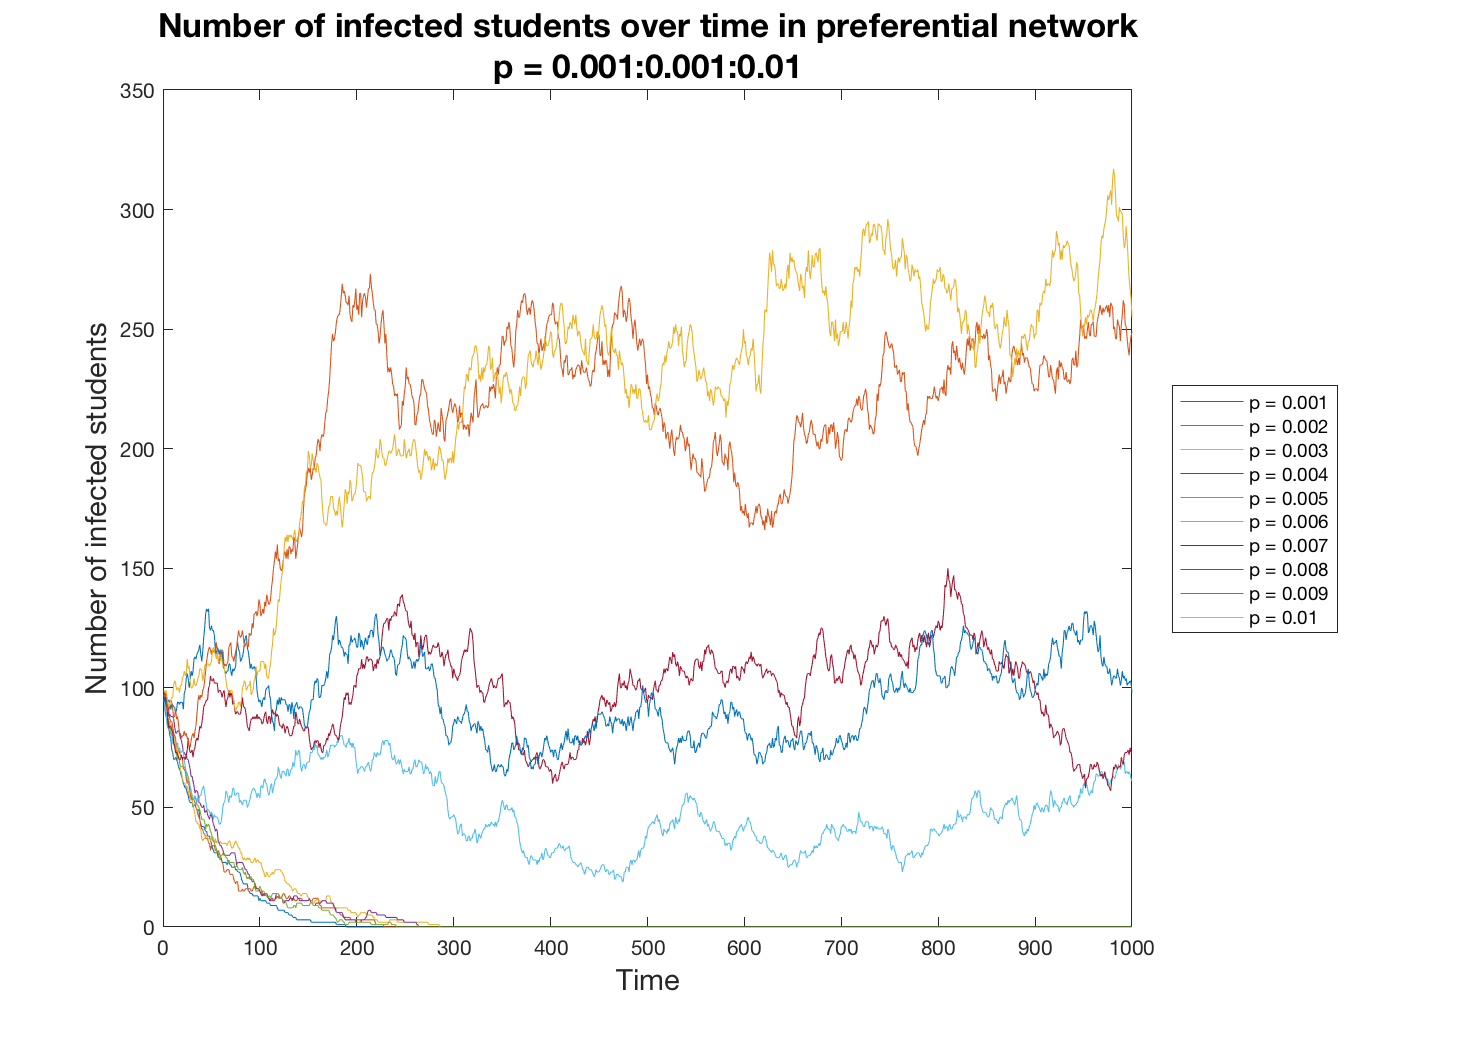
\includegraphics[width = 16 cm, height = 13cm]{pnwinf.png}
\caption{Number of infected individuals against time with different p}
\label{fig:pnwinf}
\end{figure}

\begin{figure}[H] %loglog plot for degree
\centering
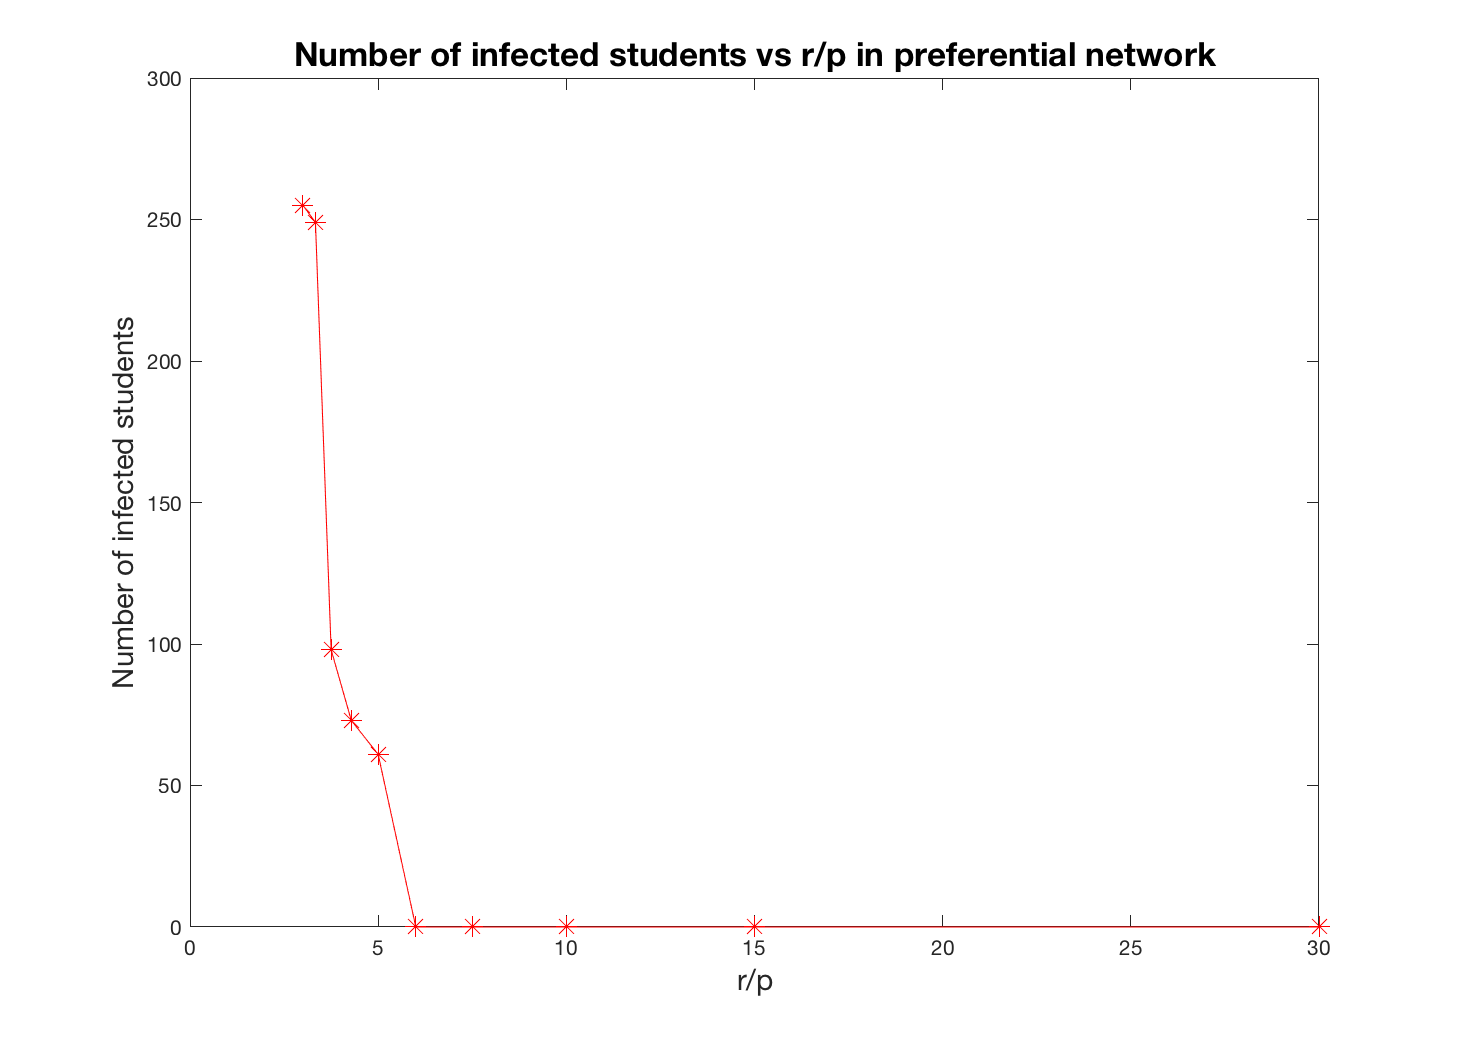
\includegraphics[width = 16 cm, height = 13cm]{pnwprp.png}
\caption{Number of infected individuals against time with different p}
\label{fig:pnwprp}
\end{figure}




%%%%%%%%%%%%%%%%%part 4
\newpage
\section{Flocks and Predators}
\doublespacing

\subsection{Alignment}

Run the Vicsek alignment model with 40 particles, domain size L = 10, angular noise e = 0.5, for 200 time steps, at each time, the direction of a particle is the average direction of its 4 nearest neighbours. The alignment varies from individual runs of the model, but generally, the particles all move towards the same direction very quick.

\begin{figure}[H] %Alignment
\centering
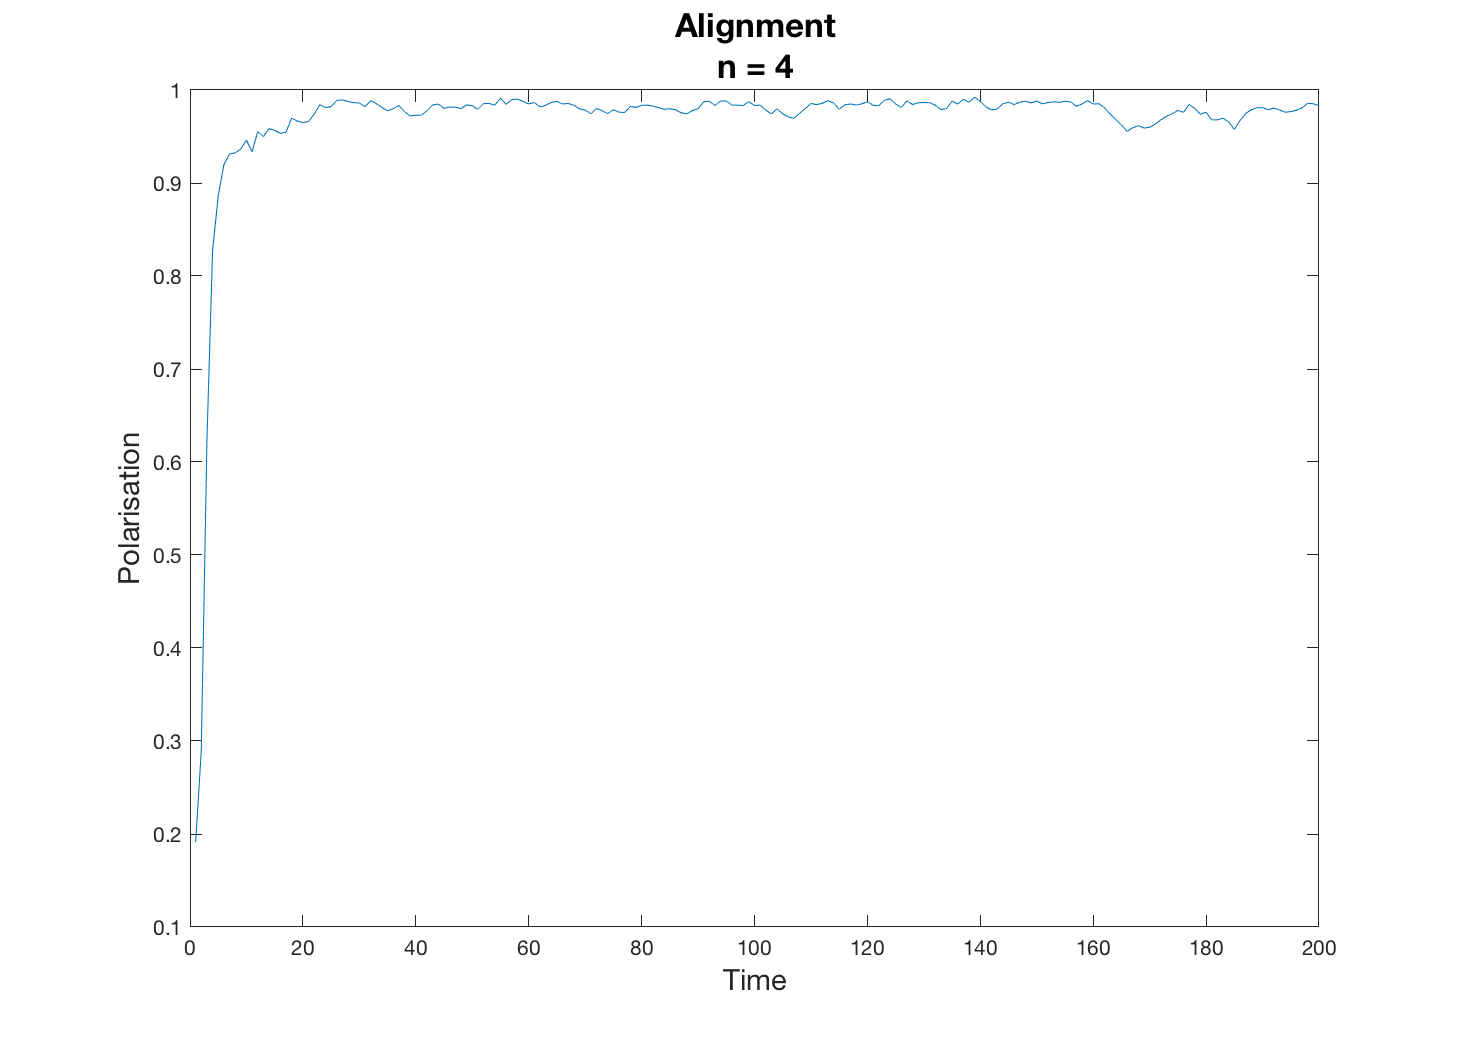
\includegraphics[width = 16 cm, height = 13cm]{palign.png}
\caption{Alignment (4 nearest neighbour)}
\label{fig:align}
\end{figure}



\subsection{Add a small force }

We add a small force that pulls the particles toward the center of mass. with coefficient 0.1. and we run the model with 40 particles, domain size L = 10, angular noise e = 0.1:0.1:6, nearest neighbour (n) = 1: 1:39 for 200 time steps with 10 replication. Then take average of the last half of the alignment. we get the heat map showing the steady-state alignment change with n and e.
\begin{figure}[H] %heatmap
\centering
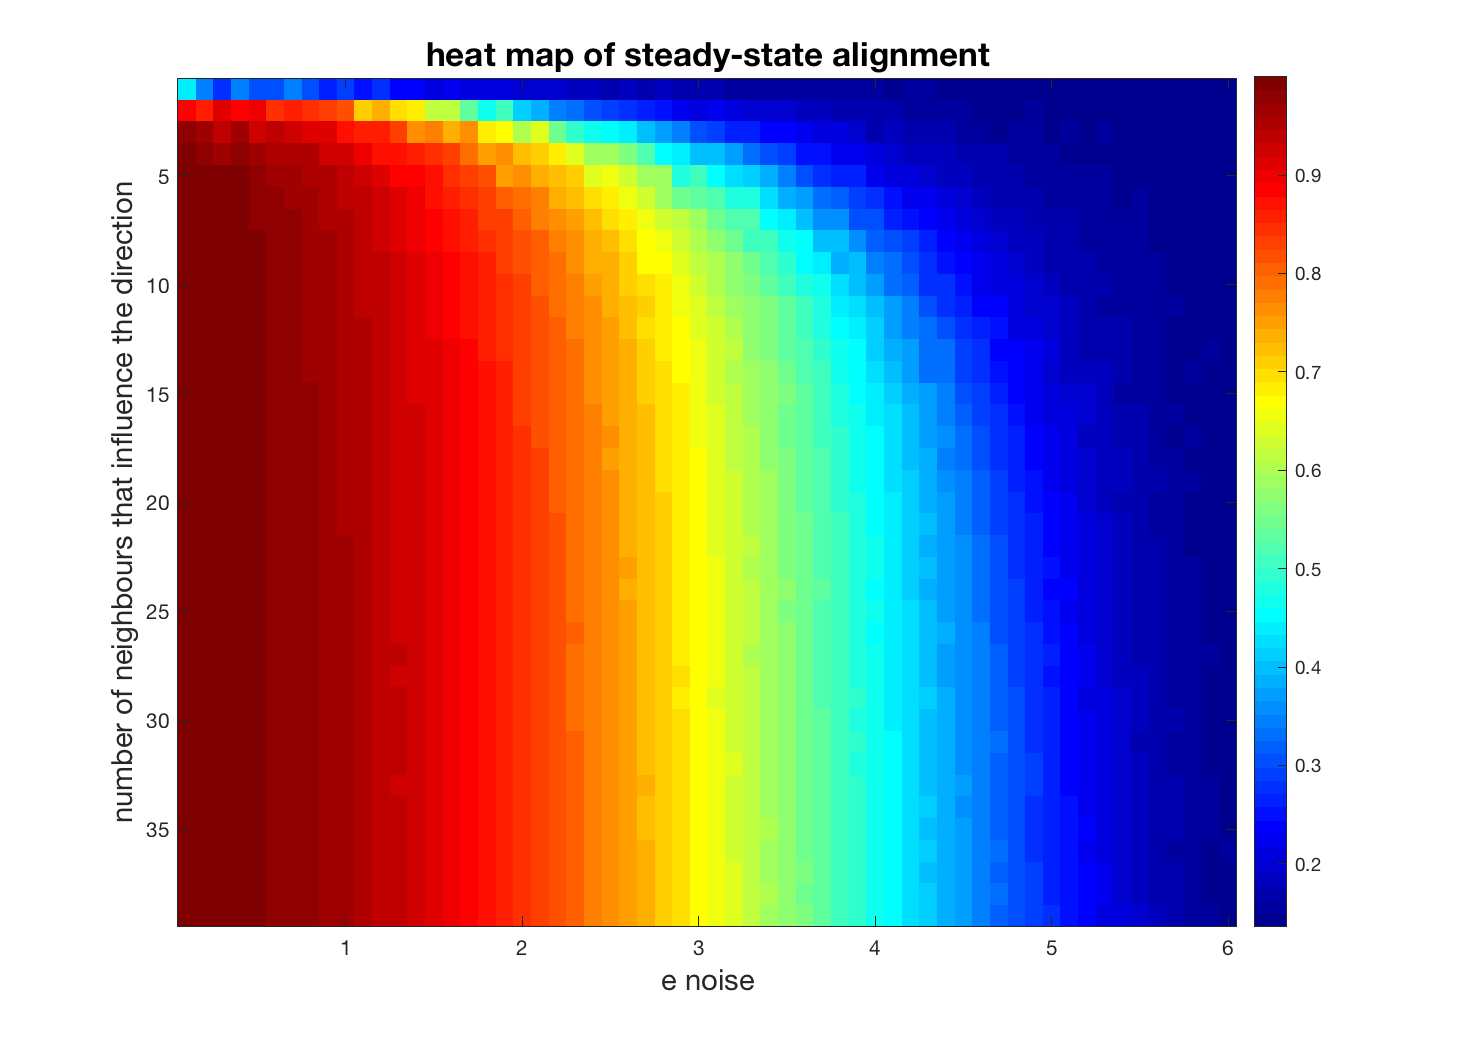
\includegraphics[width = 16 cm, height = 13cm]{heatmap.png}
\caption{Heat map of steady state alignment}
\label{fig:hm}
\end{figure}


\subsection{Predator}

We add a small force that pulls the particles toward the center of mass. with coefficient 0.1. and we run the model with 40 particles, domain size L = 10, angular noise e = 0.1:0.1:6, nearest neighbour (n) = 1: 1:39 for 200 time steps with 10 replication. Then take average of the last half of the alignment. we get the heat map showing the steady-state alignment change with n and e.
\begin{figure}[H] %heatmap
\centering
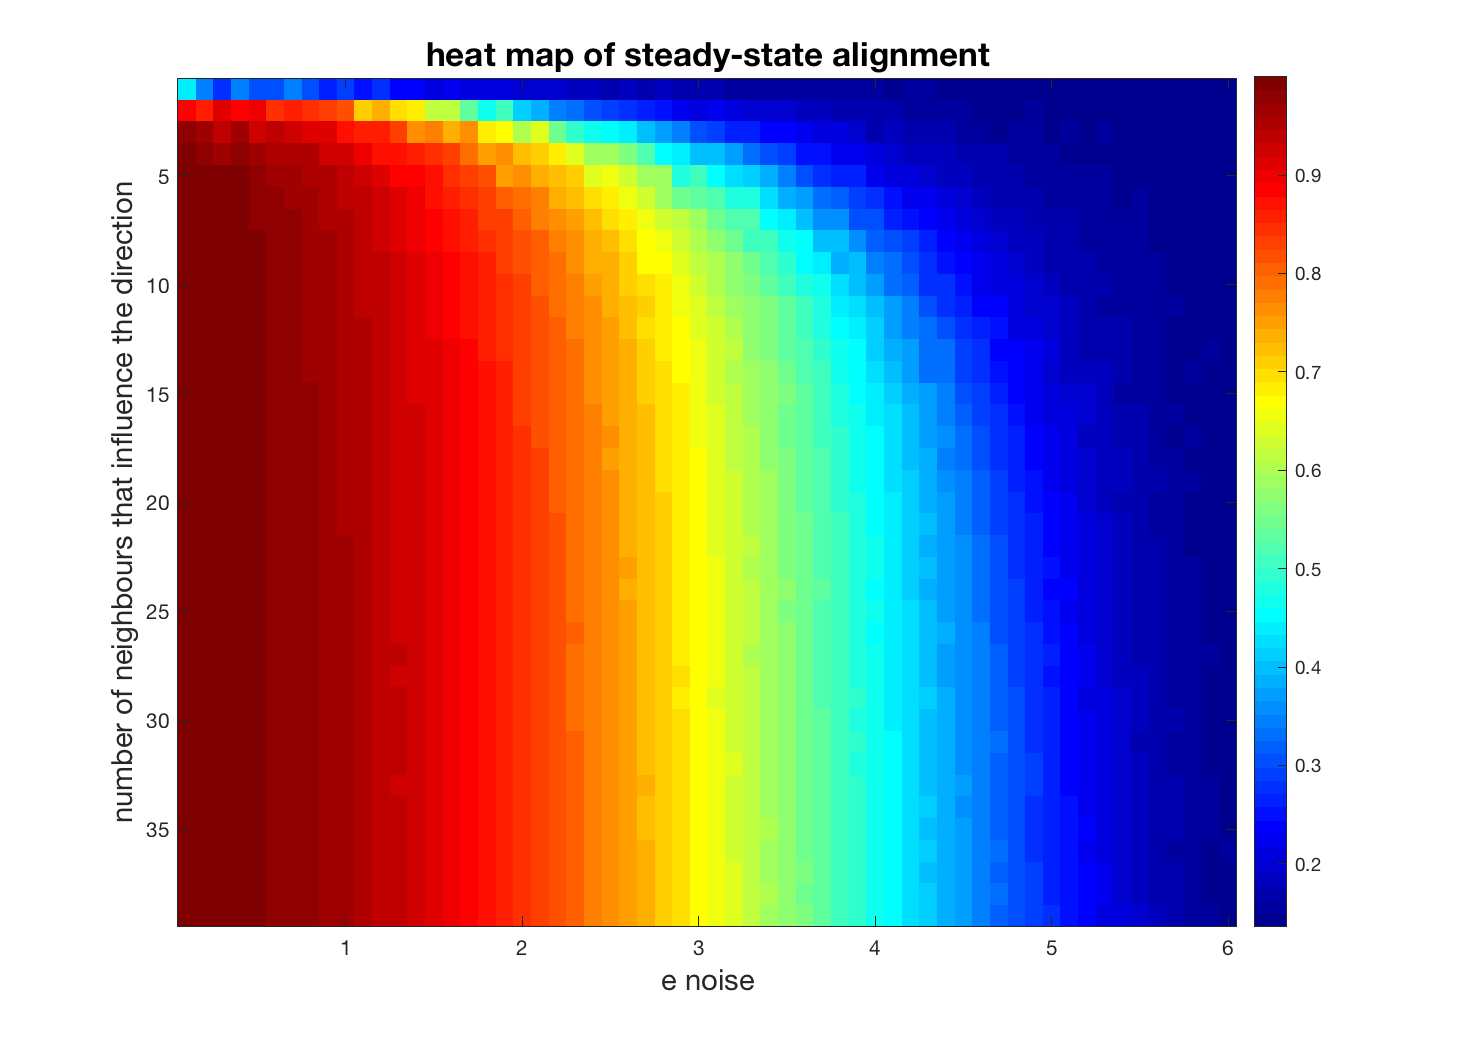
\includegraphics[width = 16 cm, height = 13cm]{heatmap.png}
\caption{Heat map of steady state alignment}
\label{fig:hm}
\end{figure}




%%%%%%%%%%%%%%%%%%
%%%%%%%%%%%%%%%%%
%%%%%%%%%%%%%%%%%appendix
\newpage
\section{Appendix}

\subsection{1firing brain code in matlab}
\singlespacing
\begin{itemize}
\item {\large simulate single time of fire brain}
\lstinputlisting{firebrain1.m}
\vspace{1cm}

\item {\large transition function}
\lstinputlisting{transit.m}
\vspace{1cm}

\item {\large initial state}
\lstinputlisting{random_start.m}
\vspace{1cm}

\item {\large simulate 100 times of firing brain}
\lstinputlisting{firebrain1_simulate100.m}
\vspace{1cm}

\item {\large cell that move forward at one cell per time preserving the same shape}
\lstinputlisting{task2_1.m}
\vspace{1cm}

\item {\large cell that move forwad at one cell per time, launching other shapes behind them}
\lstinputlisting{task2_2a.m}
\vspace{1cm}

\item {\large move forward at a rate of less than one cell per time step}
\lstinputlisting{task2_3.m}
\vspace{1cm}

\item {\large oscillate shape}
\lstinputlisting{task2_4.m}
\vspace{1cm}


\item {\large my cellular automata}
\lstinputlisting{reproduceown.m}
\vspace{1cm}

\item {\large my cellular automata transit}
\lstinputlisting{transitown.m}
\vspace{1cm}


\end{itemize}



\subsection{Spread of memes}

\singlespacing
\begin{itemize}

\item{\large simulation of spread of memes}
\lstinputlisting{sim_meme1.m}
\vspace{1cm}

\item{\large run single spread of memes }
\lstinputlisting{runmeme.m}
\vspace{1cm}

\item{\large mean field model}
\lstinputlisting{sim_meme_model.m}
\vspace{1cm}

\item{\large phase transition}
\lstinputlisting{sim_meme_phase.m}
\vspace{1cm}


\item{\large probability for at least 25\% are sharing}
\lstinputlisting{plargethan250.m}
\vspace{1cm}


\item{\large simulation of spread of memes with new rules}
\lstinputlisting{sim_meme2.m}
\vspace{1cm}

\item{\large run single spread of memes }
\lstinputlisting{runmeme_newbored.m}
\vspace{1cm}

\item{\large mean field model}
\lstinputlisting{sim_meme_model2.m}
\vspace{1cm}

\item{\large phase transition for new rules}
\lstinputlisting{sim_meme_phase2.m}
\vspace{1cm}

\item{\large lattice simulation for memes}
\lstinputlisting{memegrid.m}
\vspace{1cm}

\item{\large transition function for memes}
\lstinputlisting{transit_meme.m}
\vspace{1cm}


\end{itemize}


\end{document}